% =============================================================================
% 05-addressing-cpu-bus.tex — Week 5: Addressing Modes, CPU Organization,
% Single/Multiple Bus Organization
%
% Course: Computer Organization and Architecture (PCC CS-401)
% Anchor reading: Hamacher Ch. 7 (addressing modes, bus organization);
%                 Mano Ch. 7 (single-bus datapath, RTL)
%
% Compile with: /compile-latex CS401/05-addressing-cpu-bus
% =============================================================================

\documentclass[aspectratio=169]{beamer}
% =============================================================================
% Preambles/header.tex — shared LaTeX/Beamer preamble for this project
%
% Use from a Beamer lecture by prepending:
%     % =============================================================================
% Preambles/header.tex — shared LaTeX/Beamer preamble for this project
%
% Use from a Beamer lecture by prepending:
%     % =============================================================================
% Preambles/header.tex — shared LaTeX/Beamer preamble for this project
%
% Use from a Beamer lecture by prepending:
%     \input{header}
% and compiling with TEXINPUTS=../Preambles:$TEXINPUTS (the /compile-latex
% skill does this automatically).
%
% PALETTE CONTRACT. Color names defined here MUST match the names in
% Quarto/theme-template.scss so Beamer and Quarto renderings use the same
% palette. The scripts/check-palette-sync.sh script enforces this.
%
% To customize: edit the HEX values below AND the matching $variable in
% Quarto/theme-template.scss, then run scripts/check-palette-sync.sh.
%
% TITLE PAGE. A formal, serif (Libertine) title-page template is defined in
% the Beamer-only block below (\setbeamertemplate{title page}) -- title,
% subtitle, a thin gold rule, then \author/\institute/\date. Frametitle and
% body text remain on Beamer's sans-serif default. No SCSS counterpart is
% needed for this (font/layout only, no new colors).
% =============================================================================

% -----------------------------------------------------------------------------
% Engine detection + encoding
%
% Our /compile-latex skill uses XeLaTeX, where inputenc is unnecessary and
% can produce encoding warnings. Only load inputenc under pdfTeX.
% -----------------------------------------------------------------------------
\usepackage{iftex}
\ifPDFTeX
  \usepackage[utf8]{inputenc}
\fi

\usepackage{amsmath, amssymb, amsthm}
\usepackage{booktabs}
\usepackage{graphicx}

% -----------------------------------------------------------------------------
% Serif face for the title page (formal/academic look). Linux Libertine is
% XeLaTeX- and pdfTeX-safe and redefines \rmdefault, so \rmfamily picks it up
% everywhere \rmfamily is used explicitly. Body text and frametitles stay on
% Beamer's own sans-serif default (unaffected) -- only the title-page
% \setbeamerfont{...} overrides below opt in to \rmfamily.
% -----------------------------------------------------------------------------
\usepackage{libertine}

% -----------------------------------------------------------------------------
% PALETTE — mirrors Quarto/theme-template.scss variable names.
% Load xcolor and define colors BEFORE anything that references them
% (notably hyperref, hypersetup, and the Beamer color assignments).
% -----------------------------------------------------------------------------
\usepackage{xcolor}

\definecolor{primary-blue}{HTML}{012169}      % headings, accents
\definecolor{primary-gold}{HTML}{B9975B}      % emphasis, borders
\definecolor{highlight-yellow}{HTML}{F2A900}  % markers, alerts
\definecolor{light-bg}{HTML}{E8EDF5}          % title / section backgrounds
\definecolor{jet}{HTML}{1A1A1A}               % body text

% Semantic colors (used in diagrams and annotations)
\definecolor{positive}{HTML}{15803D}          % good / observed / identified
\definecolor{negative}{HTML}{B91C1C}          % bad / problematic / bias
\definecolor{neutral}{HTML}{525252}           % reference / context

% Highlight accents (match .hi-* classes in the SCSS)
\definecolor{hi-slate}{HTML}{314F4F}
\definecolor{hi-green}{HTML}{2E8B57}
\definecolor{hi-red}{HTML}{C41E3A}

% Semantic aliases so skill templates and snippets can write
% \textcolor{accent}{...} without hard-coding "primary-blue".
\colorlet{accent}{primary-blue}
\colorlet{accent2}{primary-gold}

% -----------------------------------------------------------------------------
% Hyperref — loaded AFTER xcolor + palette so link colors resolve.
% -----------------------------------------------------------------------------
\usepackage{hyperref}
\hypersetup{colorlinks=true, linkcolor=primary-blue, urlcolor=primary-blue,
            citecolor=primary-blue, pdfborder={0 0 0}}

% -----------------------------------------------------------------------------
% Course code — set once per deck (after \input{header}, before \begin{document})
% via \coursecode{CS401}. Shown in the footer on every slide so a deck's course
% is identifiable without opening the title page. Empty by default.
% -----------------------------------------------------------------------------
\makeatletter
\newcommand{\coursecode}[1]{\gdef\@coursecodetext{#1}}
\gdef\@coursecodetext{}
\makeatother

% -----------------------------------------------------------------------------
% Beamer theme assignments (only apply under Beamer).
%
% We detect Beamer via \@ifclassloaded{beamer}, which is the documented,
% non-internal way. This must be wrapped in \makeatletter/\makeatother
% because \@ifclassloaded contains an @-catcode character.
% -----------------------------------------------------------------------------
\makeatletter
\@ifclassloaded{beamer}{%
  \usefonttheme{professionalfonts}
  \setbeamercolor{structure}{fg=primary-blue}
  \setbeamercolor{frametitle}{fg=primary-blue}
  \setbeamercolor{title}{fg=primary-blue}
  \setbeamercolor{subtitle}{fg=primary-gold}
  \setbeamercolor{author}{fg=primary-blue}
  \setbeamercolor{institute}{fg=neutral}
  \setbeamercolor{date}{fg=primary-gold}
  \setbeamercolor{itemize item}{fg=primary-blue}
  \setbeamercolor{itemize subitem}{fg=primary-gold}
  \setbeamercolor{alerted text}{fg=primary-gold}
  \setbeamercolor{block title}{fg=white, bg=primary-blue}
  \setbeamercolor{block body}{bg=light-bg}
  % Semantic block variants: block=definition/concept (blue), exampleblock=
  % worked example (green/positive), alertblock=key takeaway or caution (gold).
  % Keep to <=2 colored boxes per slide across ALL three variants (INV-7).
  \setbeamercolor{block title example}{fg=white, bg=positive}
  \setbeamercolor{block body example}{bg=light-bg}
  \setbeamercolor{block title alerted}{fg=white, bg=primary-gold}
  \setbeamercolor{block body alerted}{bg=light-bg}

  % ---------------------------------------------------------------------------
  % Formal title page: serif (Libertine, via \rmfamily) for title-page
  % elements only. Body text, itemize, and frametitle are intentionally left
  % on Beamer's sans-serif default -- \usebeamerfont{title} is also what
  % \transitionslide (below) uses for its big centered text, so section
  % transitions pick up the same serif treatment for free.
  % ---------------------------------------------------------------------------
  \setbeamerfont{title}{family=\rmfamily, series=\bfseries, size=\Large}
  \setbeamerfont{subtitle}{family=\rmfamily, shape=\itshape, size=\normalsize}
  \setbeamerfont{author}{family=\rmfamily, size=\normalsize}
  \setbeamerfont{institute}{family=\rmfamily, size=\scriptsize}
  \setbeamerfont{date}{family=\rmfamily, size=\scriptsize}

  \setbeamertemplate{title page}{
    \vfill
    \begin{center}
      {\usebeamerfont{title}\usebeamercolor[fg]{title}\inserttitle\par}
      \vspace{0.15cm}
      {\usebeamerfont{subtitle}\usebeamercolor[fg]{subtitle}\insertsubtitle\par}
      \vspace{0.45cm}
      {\color{primary-gold}\rule{0.42\textwidth}{0.6pt}\par}
      \vspace{0.45cm}
      {\usebeamerfont{author}\usebeamercolor[fg]{author}\insertauthor\par}
      \vspace{0.35cm}
      {\usebeamerfont{institute}\usebeamercolor[fg]{institute}\insertinstitute\par}
      \vspace{0.35cm}
      {\usebeamerfont{date}\usebeamercolor[fg]{date}\insertdate\par}
    \end{center}
    \vfill
  }

  % Minimal footer: course code (left) + page X / N (right), no navigation clutter
  \setbeamertemplate{navigation symbols}{}
  \setbeamertemplate{footline}{%
    \color{neutral}\footnotesize\hspace{0.7em}\@coursecodetext\hfill
    \insertframenumber/\inserttotalframenumber\hspace{0.7em}\vspace{0.3em}}
}{}
\makeatother

% -----------------------------------------------------------------------------
% TikZ setup — libraries the snippet gallery uses
% -----------------------------------------------------------------------------
\usepackage{tikz}
\usetikzlibrary{arrows.meta, positioning, calc, decorations.pathreplacing,
                fit, shapes.geometric, backgrounds}

% Shared TikZ styles — snippets and hand-written diagrams can pick these up
% via `\begin{tikzpicture}[every node/.style={...}]` or by naming specific
% styles (e.g., `\node[dag-node] (X) at (0,0) {X};`).
\tikzset{
  % Node styles for causal DAGs and similar
  dag-node/.style = {
    draw=primary-blue, fill=light-bg, rounded corners=2pt,
    minimum width=1.2cm, minimum height=0.9cm, align=center, font=\small
  },
  decision-node/.style = {
    draw=primary-gold, fill=white, diamond, aspect=1.8,
    minimum width=1.8cm, minimum height=1.2cm, align=center, font=\small,
    inner sep=1pt
  },
  % Edge styles — observed vs counterfactual
  observed-edge/.style = {-{Latex[length=2.5mm]}, thick, draw=jet},
  counterfactual-edge/.style = {-{Latex[length=2.5mm]}, thick, draw=neutral, dashed},
  confound-edge/.style = {-{Latex[length=2.5mm]}, thick, draw=negative, dashed},
  % Data-point styles for plots
  observed-dot/.style = {fill=primary-blue, draw=primary-blue, circle, inner sep=1.2pt},
  counterfactual-dot/.style = {fill=white, draw=neutral, circle, inner sep=1.2pt}
}

% -----------------------------------------------------------------------------
% Convenience macros
% -----------------------------------------------------------------------------
\newcommand{\muted}[1]{\textcolor{neutral}{#1}}
\newcommand{\key}[1]{\textcolor{primary-gold}{\textbf{#1}}}
\newcommand{\good}[1]{\textcolor{positive}{#1}}
\newcommand{\bad}[1]{\textcolor{negative}{#1}}

% Standout frame macro: full-bleed dark background for section transitions.
% Beamer-only (uses \begin{frame}/\setbeamercolor/\usebeamerfont) -- do not
% call from an article-class file (e.g. Notes/<CODE>/*-notes.tex). \muted,
% \key, \good, \bad, and \coursecode above are plain xcolor/gdef and are
% safe to use from either class; verified when Notes/article-class support
% was added.
% Expand: \transitionslide{Your transition title}
\newcommand{\transitionslide}[1]{%
  \begingroup
  \setbeamercolor{background canvas}{bg=primary-blue}
  \begin{frame}[plain]
    \centering
    \vfill
    {\usebeamerfont{title}\color{white}\Large #1\par}
    \vfill
  \end{frame}
  \endgroup
}

% and compiling with TEXINPUTS=../Preambles:$TEXINPUTS (the /compile-latex
% skill does this automatically).
%
% PALETTE CONTRACT. Color names defined here MUST match the names in
% Quarto/theme-template.scss so Beamer and Quarto renderings use the same
% palette. The scripts/check-palette-sync.sh script enforces this.
%
% To customize: edit the HEX values below AND the matching $variable in
% Quarto/theme-template.scss, then run scripts/check-palette-sync.sh.
%
% TITLE PAGE. A formal, serif (Libertine) title-page template is defined in
% the Beamer-only block below (\setbeamertemplate{title page}) -- title,
% subtitle, a thin gold rule, then \author/\institute/\date. Frametitle and
% body text remain on Beamer's sans-serif default. No SCSS counterpart is
% needed for this (font/layout only, no new colors).
% =============================================================================

% -----------------------------------------------------------------------------
% Engine detection + encoding
%
% Our /compile-latex skill uses XeLaTeX, where inputenc is unnecessary and
% can produce encoding warnings. Only load inputenc under pdfTeX.
% -----------------------------------------------------------------------------
\usepackage{iftex}
\ifPDFTeX
  \usepackage[utf8]{inputenc}
\fi

\usepackage{amsmath, amssymb, amsthm}
\usepackage{booktabs}
\usepackage{graphicx}

% -----------------------------------------------------------------------------
% Serif face for the title page (formal/academic look). Linux Libertine is
% XeLaTeX- and pdfTeX-safe and redefines \rmdefault, so \rmfamily picks it up
% everywhere \rmfamily is used explicitly. Body text and frametitles stay on
% Beamer's own sans-serif default (unaffected) -- only the title-page
% \setbeamerfont{...} overrides below opt in to \rmfamily.
% -----------------------------------------------------------------------------
\usepackage{libertine}

% -----------------------------------------------------------------------------
% PALETTE — mirrors Quarto/theme-template.scss variable names.
% Load xcolor and define colors BEFORE anything that references them
% (notably hyperref, hypersetup, and the Beamer color assignments).
% -----------------------------------------------------------------------------
\usepackage{xcolor}

\definecolor{primary-blue}{HTML}{012169}      % headings, accents
\definecolor{primary-gold}{HTML}{B9975B}      % emphasis, borders
\definecolor{highlight-yellow}{HTML}{F2A900}  % markers, alerts
\definecolor{light-bg}{HTML}{E8EDF5}          % title / section backgrounds
\definecolor{jet}{HTML}{1A1A1A}               % body text

% Semantic colors (used in diagrams and annotations)
\definecolor{positive}{HTML}{15803D}          % good / observed / identified
\definecolor{negative}{HTML}{B91C1C}          % bad / problematic / bias
\definecolor{neutral}{HTML}{525252}           % reference / context

% Highlight accents (match .hi-* classes in the SCSS)
\definecolor{hi-slate}{HTML}{314F4F}
\definecolor{hi-green}{HTML}{2E8B57}
\definecolor{hi-red}{HTML}{C41E3A}

% Semantic aliases so skill templates and snippets can write
% \textcolor{accent}{...} without hard-coding "primary-blue".
\colorlet{accent}{primary-blue}
\colorlet{accent2}{primary-gold}

% -----------------------------------------------------------------------------
% Hyperref — loaded AFTER xcolor + palette so link colors resolve.
% -----------------------------------------------------------------------------
\usepackage{hyperref}
\hypersetup{colorlinks=true, linkcolor=primary-blue, urlcolor=primary-blue,
            citecolor=primary-blue, pdfborder={0 0 0}}

% -----------------------------------------------------------------------------
% Course code — set once per deck (after % =============================================================================
% Preambles/header.tex — shared LaTeX/Beamer preamble for this project
%
% Use from a Beamer lecture by prepending:
%     \input{header}
% and compiling with TEXINPUTS=../Preambles:$TEXINPUTS (the /compile-latex
% skill does this automatically).
%
% PALETTE CONTRACT. Color names defined here MUST match the names in
% Quarto/theme-template.scss so Beamer and Quarto renderings use the same
% palette. The scripts/check-palette-sync.sh script enforces this.
%
% To customize: edit the HEX values below AND the matching $variable in
% Quarto/theme-template.scss, then run scripts/check-palette-sync.sh.
%
% TITLE PAGE. A formal, serif (Libertine) title-page template is defined in
% the Beamer-only block below (\setbeamertemplate{title page}) -- title,
% subtitle, a thin gold rule, then \author/\institute/\date. Frametitle and
% body text remain on Beamer's sans-serif default. No SCSS counterpart is
% needed for this (font/layout only, no new colors).
% =============================================================================

% -----------------------------------------------------------------------------
% Engine detection + encoding
%
% Our /compile-latex skill uses XeLaTeX, where inputenc is unnecessary and
% can produce encoding warnings. Only load inputenc under pdfTeX.
% -----------------------------------------------------------------------------
\usepackage{iftex}
\ifPDFTeX
  \usepackage[utf8]{inputenc}
\fi

\usepackage{amsmath, amssymb, amsthm}
\usepackage{booktabs}
\usepackage{graphicx}

% -----------------------------------------------------------------------------
% Serif face for the title page (formal/academic look). Linux Libertine is
% XeLaTeX- and pdfTeX-safe and redefines \rmdefault, so \rmfamily picks it up
% everywhere \rmfamily is used explicitly. Body text and frametitles stay on
% Beamer's own sans-serif default (unaffected) -- only the title-page
% \setbeamerfont{...} overrides below opt in to \rmfamily.
% -----------------------------------------------------------------------------
\usepackage{libertine}

% -----------------------------------------------------------------------------
% PALETTE — mirrors Quarto/theme-template.scss variable names.
% Load xcolor and define colors BEFORE anything that references them
% (notably hyperref, hypersetup, and the Beamer color assignments).
% -----------------------------------------------------------------------------
\usepackage{xcolor}

\definecolor{primary-blue}{HTML}{012169}      % headings, accents
\definecolor{primary-gold}{HTML}{B9975B}      % emphasis, borders
\definecolor{highlight-yellow}{HTML}{F2A900}  % markers, alerts
\definecolor{light-bg}{HTML}{E8EDF5}          % title / section backgrounds
\definecolor{jet}{HTML}{1A1A1A}               % body text

% Semantic colors (used in diagrams and annotations)
\definecolor{positive}{HTML}{15803D}          % good / observed / identified
\definecolor{negative}{HTML}{B91C1C}          % bad / problematic / bias
\definecolor{neutral}{HTML}{525252}           % reference / context

% Highlight accents (match .hi-* classes in the SCSS)
\definecolor{hi-slate}{HTML}{314F4F}
\definecolor{hi-green}{HTML}{2E8B57}
\definecolor{hi-red}{HTML}{C41E3A}

% Semantic aliases so skill templates and snippets can write
% \textcolor{accent}{...} without hard-coding "primary-blue".
\colorlet{accent}{primary-blue}
\colorlet{accent2}{primary-gold}

% -----------------------------------------------------------------------------
% Hyperref — loaded AFTER xcolor + palette so link colors resolve.
% -----------------------------------------------------------------------------
\usepackage{hyperref}
\hypersetup{colorlinks=true, linkcolor=primary-blue, urlcolor=primary-blue,
            citecolor=primary-blue, pdfborder={0 0 0}}

% -----------------------------------------------------------------------------
% Course code — set once per deck (after \input{header}, before \begin{document})
% via \coursecode{CS401}. Shown in the footer on every slide so a deck's course
% is identifiable without opening the title page. Empty by default.
% -----------------------------------------------------------------------------
\makeatletter
\newcommand{\coursecode}[1]{\gdef\@coursecodetext{#1}}
\gdef\@coursecodetext{}
\makeatother

% -----------------------------------------------------------------------------
% Beamer theme assignments (only apply under Beamer).
%
% We detect Beamer via \@ifclassloaded{beamer}, which is the documented,
% non-internal way. This must be wrapped in \makeatletter/\makeatother
% because \@ifclassloaded contains an @-catcode character.
% -----------------------------------------------------------------------------
\makeatletter
\@ifclassloaded{beamer}{%
  \usefonttheme{professionalfonts}
  \setbeamercolor{structure}{fg=primary-blue}
  \setbeamercolor{frametitle}{fg=primary-blue}
  \setbeamercolor{title}{fg=primary-blue}
  \setbeamercolor{subtitle}{fg=primary-gold}
  \setbeamercolor{author}{fg=primary-blue}
  \setbeamercolor{institute}{fg=neutral}
  \setbeamercolor{date}{fg=primary-gold}
  \setbeamercolor{itemize item}{fg=primary-blue}
  \setbeamercolor{itemize subitem}{fg=primary-gold}
  \setbeamercolor{alerted text}{fg=primary-gold}
  \setbeamercolor{block title}{fg=white, bg=primary-blue}
  \setbeamercolor{block body}{bg=light-bg}
  % Semantic block variants: block=definition/concept (blue), exampleblock=
  % worked example (green/positive), alertblock=key takeaway or caution (gold).
  % Keep to <=2 colored boxes per slide across ALL three variants (INV-7).
  \setbeamercolor{block title example}{fg=white, bg=positive}
  \setbeamercolor{block body example}{bg=light-bg}
  \setbeamercolor{block title alerted}{fg=white, bg=primary-gold}
  \setbeamercolor{block body alerted}{bg=light-bg}

  % ---------------------------------------------------------------------------
  % Formal title page: serif (Libertine, via \rmfamily) for title-page
  % elements only. Body text, itemize, and frametitle are intentionally left
  % on Beamer's sans-serif default -- \usebeamerfont{title} is also what
  % \transitionslide (below) uses for its big centered text, so section
  % transitions pick up the same serif treatment for free.
  % ---------------------------------------------------------------------------
  \setbeamerfont{title}{family=\rmfamily, series=\bfseries, size=\Large}
  \setbeamerfont{subtitle}{family=\rmfamily, shape=\itshape, size=\normalsize}
  \setbeamerfont{author}{family=\rmfamily, size=\normalsize}
  \setbeamerfont{institute}{family=\rmfamily, size=\scriptsize}
  \setbeamerfont{date}{family=\rmfamily, size=\scriptsize}

  \setbeamertemplate{title page}{
    \vfill
    \begin{center}
      {\usebeamerfont{title}\usebeamercolor[fg]{title}\inserttitle\par}
      \vspace{0.15cm}
      {\usebeamerfont{subtitle}\usebeamercolor[fg]{subtitle}\insertsubtitle\par}
      \vspace{0.45cm}
      {\color{primary-gold}\rule{0.42\textwidth}{0.6pt}\par}
      \vspace{0.45cm}
      {\usebeamerfont{author}\usebeamercolor[fg]{author}\insertauthor\par}
      \vspace{0.35cm}
      {\usebeamerfont{institute}\usebeamercolor[fg]{institute}\insertinstitute\par}
      \vspace{0.35cm}
      {\usebeamerfont{date}\usebeamercolor[fg]{date}\insertdate\par}
    \end{center}
    \vfill
  }

  % Minimal footer: course code (left) + page X / N (right), no navigation clutter
  \setbeamertemplate{navigation symbols}{}
  \setbeamertemplate{footline}{%
    \color{neutral}\footnotesize\hspace{0.7em}\@coursecodetext\hfill
    \insertframenumber/\inserttotalframenumber\hspace{0.7em}\vspace{0.3em}}
}{}
\makeatother

% -----------------------------------------------------------------------------
% TikZ setup — libraries the snippet gallery uses
% -----------------------------------------------------------------------------
\usepackage{tikz}
\usetikzlibrary{arrows.meta, positioning, calc, decorations.pathreplacing,
                fit, shapes.geometric, backgrounds}

% Shared TikZ styles — snippets and hand-written diagrams can pick these up
% via `\begin{tikzpicture}[every node/.style={...}]` or by naming specific
% styles (e.g., `\node[dag-node] (X) at (0,0) {X};`).
\tikzset{
  % Node styles for causal DAGs and similar
  dag-node/.style = {
    draw=primary-blue, fill=light-bg, rounded corners=2pt,
    minimum width=1.2cm, minimum height=0.9cm, align=center, font=\small
  },
  decision-node/.style = {
    draw=primary-gold, fill=white, diamond, aspect=1.8,
    minimum width=1.8cm, minimum height=1.2cm, align=center, font=\small,
    inner sep=1pt
  },
  % Edge styles — observed vs counterfactual
  observed-edge/.style = {-{Latex[length=2.5mm]}, thick, draw=jet},
  counterfactual-edge/.style = {-{Latex[length=2.5mm]}, thick, draw=neutral, dashed},
  confound-edge/.style = {-{Latex[length=2.5mm]}, thick, draw=negative, dashed},
  % Data-point styles for plots
  observed-dot/.style = {fill=primary-blue, draw=primary-blue, circle, inner sep=1.2pt},
  counterfactual-dot/.style = {fill=white, draw=neutral, circle, inner sep=1.2pt}
}

% -----------------------------------------------------------------------------
% Convenience macros
% -----------------------------------------------------------------------------
\newcommand{\muted}[1]{\textcolor{neutral}{#1}}
\newcommand{\key}[1]{\textcolor{primary-gold}{\textbf{#1}}}
\newcommand{\good}[1]{\textcolor{positive}{#1}}
\newcommand{\bad}[1]{\textcolor{negative}{#1}}

% Standout frame macro: full-bleed dark background for section transitions.
% Beamer-only (uses \begin{frame}/\setbeamercolor/\usebeamerfont) -- do not
% call from an article-class file (e.g. Notes/<CODE>/*-notes.tex). \muted,
% \key, \good, \bad, and \coursecode above are plain xcolor/gdef and are
% safe to use from either class; verified when Notes/article-class support
% was added.
% Expand: \transitionslide{Your transition title}
\newcommand{\transitionslide}[1]{%
  \begingroup
  \setbeamercolor{background canvas}{bg=primary-blue}
  \begin{frame}[plain]
    \centering
    \vfill
    {\usebeamerfont{title}\color{white}\Large #1\par}
    \vfill
  \end{frame}
  \endgroup
}
, before \begin{document})
% via \coursecode{CS401}. Shown in the footer on every slide so a deck's course
% is identifiable without opening the title page. Empty by default.
% -----------------------------------------------------------------------------
\makeatletter
\newcommand{\coursecode}[1]{\gdef\@coursecodetext{#1}}
\gdef\@coursecodetext{}
\makeatother

% -----------------------------------------------------------------------------
% Beamer theme assignments (only apply under Beamer).
%
% We detect Beamer via \@ifclassloaded{beamer}, which is the documented,
% non-internal way. This must be wrapped in \makeatletter/\makeatother
% because \@ifclassloaded contains an @-catcode character.
% -----------------------------------------------------------------------------
\makeatletter
\@ifclassloaded{beamer}{%
  \usefonttheme{professionalfonts}
  \setbeamercolor{structure}{fg=primary-blue}
  \setbeamercolor{frametitle}{fg=primary-blue}
  \setbeamercolor{title}{fg=primary-blue}
  \setbeamercolor{subtitle}{fg=primary-gold}
  \setbeamercolor{author}{fg=primary-blue}
  \setbeamercolor{institute}{fg=neutral}
  \setbeamercolor{date}{fg=primary-gold}
  \setbeamercolor{itemize item}{fg=primary-blue}
  \setbeamercolor{itemize subitem}{fg=primary-gold}
  \setbeamercolor{alerted text}{fg=primary-gold}
  \setbeamercolor{block title}{fg=white, bg=primary-blue}
  \setbeamercolor{block body}{bg=light-bg}
  % Semantic block variants: block=definition/concept (blue), exampleblock=
  % worked example (green/positive), alertblock=key takeaway or caution (gold).
  % Keep to <=2 colored boxes per slide across ALL three variants (INV-7).
  \setbeamercolor{block title example}{fg=white, bg=positive}
  \setbeamercolor{block body example}{bg=light-bg}
  \setbeamercolor{block title alerted}{fg=white, bg=primary-gold}
  \setbeamercolor{block body alerted}{bg=light-bg}

  % ---------------------------------------------------------------------------
  % Formal title page: serif (Libertine, via \rmfamily) for title-page
  % elements only. Body text, itemize, and frametitle are intentionally left
  % on Beamer's sans-serif default -- \usebeamerfont{title} is also what
  % \transitionslide (below) uses for its big centered text, so section
  % transitions pick up the same serif treatment for free.
  % ---------------------------------------------------------------------------
  \setbeamerfont{title}{family=\rmfamily, series=\bfseries, size=\Large}
  \setbeamerfont{subtitle}{family=\rmfamily, shape=\itshape, size=\normalsize}
  \setbeamerfont{author}{family=\rmfamily, size=\normalsize}
  \setbeamerfont{institute}{family=\rmfamily, size=\scriptsize}
  \setbeamerfont{date}{family=\rmfamily, size=\scriptsize}

  \setbeamertemplate{title page}{
    \vfill
    \begin{center}
      {\usebeamerfont{title}\usebeamercolor[fg]{title}\inserttitle\par}
      \vspace{0.15cm}
      {\usebeamerfont{subtitle}\usebeamercolor[fg]{subtitle}\insertsubtitle\par}
      \vspace{0.45cm}
      {\color{primary-gold}\rule{0.42\textwidth}{0.6pt}\par}
      \vspace{0.45cm}
      {\usebeamerfont{author}\usebeamercolor[fg]{author}\insertauthor\par}
      \vspace{0.35cm}
      {\usebeamerfont{institute}\usebeamercolor[fg]{institute}\insertinstitute\par}
      \vspace{0.35cm}
      {\usebeamerfont{date}\usebeamercolor[fg]{date}\insertdate\par}
    \end{center}
    \vfill
  }

  % Minimal footer: course code (left) + page X / N (right), no navigation clutter
  \setbeamertemplate{navigation symbols}{}
  \setbeamertemplate{footline}{%
    \color{neutral}\footnotesize\hspace{0.7em}\@coursecodetext\hfill
    \insertframenumber/\inserttotalframenumber\hspace{0.7em}\vspace{0.3em}}
}{}
\makeatother

% -----------------------------------------------------------------------------
% TikZ setup — libraries the snippet gallery uses
% -----------------------------------------------------------------------------
\usepackage{tikz}
\usetikzlibrary{arrows.meta, positioning, calc, decorations.pathreplacing,
                fit, shapes.geometric, backgrounds}

% Shared TikZ styles — snippets and hand-written diagrams can pick these up
% via `\begin{tikzpicture}[every node/.style={...}]` or by naming specific
% styles (e.g., `\node[dag-node] (X) at (0,0) {X};`).
\tikzset{
  % Node styles for causal DAGs and similar
  dag-node/.style = {
    draw=primary-blue, fill=light-bg, rounded corners=2pt,
    minimum width=1.2cm, minimum height=0.9cm, align=center, font=\small
  },
  decision-node/.style = {
    draw=primary-gold, fill=white, diamond, aspect=1.8,
    minimum width=1.8cm, minimum height=1.2cm, align=center, font=\small,
    inner sep=1pt
  },
  % Edge styles — observed vs counterfactual
  observed-edge/.style = {-{Latex[length=2.5mm]}, thick, draw=jet},
  counterfactual-edge/.style = {-{Latex[length=2.5mm]}, thick, draw=neutral, dashed},
  confound-edge/.style = {-{Latex[length=2.5mm]}, thick, draw=negative, dashed},
  % Data-point styles for plots
  observed-dot/.style = {fill=primary-blue, draw=primary-blue, circle, inner sep=1.2pt},
  counterfactual-dot/.style = {fill=white, draw=neutral, circle, inner sep=1.2pt}
}

% -----------------------------------------------------------------------------
% Convenience macros
% -----------------------------------------------------------------------------
\newcommand{\muted}[1]{\textcolor{neutral}{#1}}
\newcommand{\key}[1]{\textcolor{primary-gold}{\textbf{#1}}}
\newcommand{\good}[1]{\textcolor{positive}{#1}}
\newcommand{\bad}[1]{\textcolor{negative}{#1}}

% Standout frame macro: full-bleed dark background for section transitions.
% Beamer-only (uses \begin{frame}/\setbeamercolor/\usebeamerfont) -- do not
% call from an article-class file (e.g. Notes/<CODE>/*-notes.tex). \muted,
% \key, \good, \bad, and \coursecode above are plain xcolor/gdef and are
% safe to use from either class; verified when Notes/article-class support
% was added.
% Expand: \transitionslide{Your transition title}
\newcommand{\transitionslide}[1]{%
  \begingroup
  \setbeamercolor{background canvas}{bg=primary-blue}
  \begin{frame}[plain]
    \centering
    \vfill
    {\usebeamerfont{title}\color{white}\Large #1\par}
    \vfill
  \end{frame}
  \endgroup
}

% and compiling with TEXINPUTS=../Preambles:$TEXINPUTS (the /compile-latex
% skill does this automatically).
%
% PALETTE CONTRACT. Color names defined here MUST match the names in
% Quarto/theme-template.scss so Beamer and Quarto renderings use the same
% palette. The scripts/check-palette-sync.sh script enforces this.
%
% To customize: edit the HEX values below AND the matching $variable in
% Quarto/theme-template.scss, then run scripts/check-palette-sync.sh.
%
% TITLE PAGE. A formal, serif (Libertine) title-page template is defined in
% the Beamer-only block below (\setbeamertemplate{title page}) -- title,
% subtitle, a thin gold rule, then \author/\institute/\date. Frametitle and
% body text remain on Beamer's sans-serif default. No SCSS counterpart is
% needed for this (font/layout only, no new colors).
% =============================================================================

% -----------------------------------------------------------------------------
% Engine detection + encoding
%
% Our /compile-latex skill uses XeLaTeX, where inputenc is unnecessary and
% can produce encoding warnings. Only load inputenc under pdfTeX.
% -----------------------------------------------------------------------------
\usepackage{iftex}
\ifPDFTeX
  \usepackage[utf8]{inputenc}
\fi

\usepackage{amsmath, amssymb, amsthm}
\usepackage{booktabs}
\usepackage{graphicx}

% -----------------------------------------------------------------------------
% Serif face for the title page (formal/academic look). Linux Libertine is
% XeLaTeX- and pdfTeX-safe and redefines \rmdefault, so \rmfamily picks it up
% everywhere \rmfamily is used explicitly. Body text and frametitles stay on
% Beamer's own sans-serif default (unaffected) -- only the title-page
% \setbeamerfont{...} overrides below opt in to \rmfamily.
% -----------------------------------------------------------------------------
\usepackage{libertine}

% -----------------------------------------------------------------------------
% PALETTE — mirrors Quarto/theme-template.scss variable names.
% Load xcolor and define colors BEFORE anything that references them
% (notably hyperref, hypersetup, and the Beamer color assignments).
% -----------------------------------------------------------------------------
\usepackage{xcolor}

\definecolor{primary-blue}{HTML}{012169}      % headings, accents
\definecolor{primary-gold}{HTML}{B9975B}      % emphasis, borders
\definecolor{highlight-yellow}{HTML}{F2A900}  % markers, alerts
\definecolor{light-bg}{HTML}{E8EDF5}          % title / section backgrounds
\definecolor{jet}{HTML}{1A1A1A}               % body text

% Semantic colors (used in diagrams and annotations)
\definecolor{positive}{HTML}{15803D}          % good / observed / identified
\definecolor{negative}{HTML}{B91C1C}          % bad / problematic / bias
\definecolor{neutral}{HTML}{525252}           % reference / context

% Highlight accents (match .hi-* classes in the SCSS)
\definecolor{hi-slate}{HTML}{314F4F}
\definecolor{hi-green}{HTML}{2E8B57}
\definecolor{hi-red}{HTML}{C41E3A}

% Semantic aliases so skill templates and snippets can write
% \textcolor{accent}{...} without hard-coding "primary-blue".
\colorlet{accent}{primary-blue}
\colorlet{accent2}{primary-gold}

% -----------------------------------------------------------------------------
% Hyperref — loaded AFTER xcolor + palette so link colors resolve.
% -----------------------------------------------------------------------------
\usepackage{hyperref}
\hypersetup{colorlinks=true, linkcolor=primary-blue, urlcolor=primary-blue,
            citecolor=primary-blue, pdfborder={0 0 0}}

% -----------------------------------------------------------------------------
% Course code — set once per deck (after % =============================================================================
% Preambles/header.tex — shared LaTeX/Beamer preamble for this project
%
% Use from a Beamer lecture by prepending:
%     % =============================================================================
% Preambles/header.tex — shared LaTeX/Beamer preamble for this project
%
% Use from a Beamer lecture by prepending:
%     \input{header}
% and compiling with TEXINPUTS=../Preambles:$TEXINPUTS (the /compile-latex
% skill does this automatically).
%
% PALETTE CONTRACT. Color names defined here MUST match the names in
% Quarto/theme-template.scss so Beamer and Quarto renderings use the same
% palette. The scripts/check-palette-sync.sh script enforces this.
%
% To customize: edit the HEX values below AND the matching $variable in
% Quarto/theme-template.scss, then run scripts/check-palette-sync.sh.
%
% TITLE PAGE. A formal, serif (Libertine) title-page template is defined in
% the Beamer-only block below (\setbeamertemplate{title page}) -- title,
% subtitle, a thin gold rule, then \author/\institute/\date. Frametitle and
% body text remain on Beamer's sans-serif default. No SCSS counterpart is
% needed for this (font/layout only, no new colors).
% =============================================================================

% -----------------------------------------------------------------------------
% Engine detection + encoding
%
% Our /compile-latex skill uses XeLaTeX, where inputenc is unnecessary and
% can produce encoding warnings. Only load inputenc under pdfTeX.
% -----------------------------------------------------------------------------
\usepackage{iftex}
\ifPDFTeX
  \usepackage[utf8]{inputenc}
\fi

\usepackage{amsmath, amssymb, amsthm}
\usepackage{booktabs}
\usepackage{graphicx}

% -----------------------------------------------------------------------------
% Serif face for the title page (formal/academic look). Linux Libertine is
% XeLaTeX- and pdfTeX-safe and redefines \rmdefault, so \rmfamily picks it up
% everywhere \rmfamily is used explicitly. Body text and frametitles stay on
% Beamer's own sans-serif default (unaffected) -- only the title-page
% \setbeamerfont{...} overrides below opt in to \rmfamily.
% -----------------------------------------------------------------------------
\usepackage{libertine}

% -----------------------------------------------------------------------------
% PALETTE — mirrors Quarto/theme-template.scss variable names.
% Load xcolor and define colors BEFORE anything that references them
% (notably hyperref, hypersetup, and the Beamer color assignments).
% -----------------------------------------------------------------------------
\usepackage{xcolor}

\definecolor{primary-blue}{HTML}{012169}      % headings, accents
\definecolor{primary-gold}{HTML}{B9975B}      % emphasis, borders
\definecolor{highlight-yellow}{HTML}{F2A900}  % markers, alerts
\definecolor{light-bg}{HTML}{E8EDF5}          % title / section backgrounds
\definecolor{jet}{HTML}{1A1A1A}               % body text

% Semantic colors (used in diagrams and annotations)
\definecolor{positive}{HTML}{15803D}          % good / observed / identified
\definecolor{negative}{HTML}{B91C1C}          % bad / problematic / bias
\definecolor{neutral}{HTML}{525252}           % reference / context

% Highlight accents (match .hi-* classes in the SCSS)
\definecolor{hi-slate}{HTML}{314F4F}
\definecolor{hi-green}{HTML}{2E8B57}
\definecolor{hi-red}{HTML}{C41E3A}

% Semantic aliases so skill templates and snippets can write
% \textcolor{accent}{...} without hard-coding "primary-blue".
\colorlet{accent}{primary-blue}
\colorlet{accent2}{primary-gold}

% -----------------------------------------------------------------------------
% Hyperref — loaded AFTER xcolor + palette so link colors resolve.
% -----------------------------------------------------------------------------
\usepackage{hyperref}
\hypersetup{colorlinks=true, linkcolor=primary-blue, urlcolor=primary-blue,
            citecolor=primary-blue, pdfborder={0 0 0}}

% -----------------------------------------------------------------------------
% Course code — set once per deck (after \input{header}, before \begin{document})
% via \coursecode{CS401}. Shown in the footer on every slide so a deck's course
% is identifiable without opening the title page. Empty by default.
% -----------------------------------------------------------------------------
\makeatletter
\newcommand{\coursecode}[1]{\gdef\@coursecodetext{#1}}
\gdef\@coursecodetext{}
\makeatother

% -----------------------------------------------------------------------------
% Beamer theme assignments (only apply under Beamer).
%
% We detect Beamer via \@ifclassloaded{beamer}, which is the documented,
% non-internal way. This must be wrapped in \makeatletter/\makeatother
% because \@ifclassloaded contains an @-catcode character.
% -----------------------------------------------------------------------------
\makeatletter
\@ifclassloaded{beamer}{%
  \usefonttheme{professionalfonts}
  \setbeamercolor{structure}{fg=primary-blue}
  \setbeamercolor{frametitle}{fg=primary-blue}
  \setbeamercolor{title}{fg=primary-blue}
  \setbeamercolor{subtitle}{fg=primary-gold}
  \setbeamercolor{author}{fg=primary-blue}
  \setbeamercolor{institute}{fg=neutral}
  \setbeamercolor{date}{fg=primary-gold}
  \setbeamercolor{itemize item}{fg=primary-blue}
  \setbeamercolor{itemize subitem}{fg=primary-gold}
  \setbeamercolor{alerted text}{fg=primary-gold}
  \setbeamercolor{block title}{fg=white, bg=primary-blue}
  \setbeamercolor{block body}{bg=light-bg}
  % Semantic block variants: block=definition/concept (blue), exampleblock=
  % worked example (green/positive), alertblock=key takeaway or caution (gold).
  % Keep to <=2 colored boxes per slide across ALL three variants (INV-7).
  \setbeamercolor{block title example}{fg=white, bg=positive}
  \setbeamercolor{block body example}{bg=light-bg}
  \setbeamercolor{block title alerted}{fg=white, bg=primary-gold}
  \setbeamercolor{block body alerted}{bg=light-bg}

  % ---------------------------------------------------------------------------
  % Formal title page: serif (Libertine, via \rmfamily) for title-page
  % elements only. Body text, itemize, and frametitle are intentionally left
  % on Beamer's sans-serif default -- \usebeamerfont{title} is also what
  % \transitionslide (below) uses for its big centered text, so section
  % transitions pick up the same serif treatment for free.
  % ---------------------------------------------------------------------------
  \setbeamerfont{title}{family=\rmfamily, series=\bfseries, size=\Large}
  \setbeamerfont{subtitle}{family=\rmfamily, shape=\itshape, size=\normalsize}
  \setbeamerfont{author}{family=\rmfamily, size=\normalsize}
  \setbeamerfont{institute}{family=\rmfamily, size=\scriptsize}
  \setbeamerfont{date}{family=\rmfamily, size=\scriptsize}

  \setbeamertemplate{title page}{
    \vfill
    \begin{center}
      {\usebeamerfont{title}\usebeamercolor[fg]{title}\inserttitle\par}
      \vspace{0.15cm}
      {\usebeamerfont{subtitle}\usebeamercolor[fg]{subtitle}\insertsubtitle\par}
      \vspace{0.45cm}
      {\color{primary-gold}\rule{0.42\textwidth}{0.6pt}\par}
      \vspace{0.45cm}
      {\usebeamerfont{author}\usebeamercolor[fg]{author}\insertauthor\par}
      \vspace{0.35cm}
      {\usebeamerfont{institute}\usebeamercolor[fg]{institute}\insertinstitute\par}
      \vspace{0.35cm}
      {\usebeamerfont{date}\usebeamercolor[fg]{date}\insertdate\par}
    \end{center}
    \vfill
  }

  % Minimal footer: course code (left) + page X / N (right), no navigation clutter
  \setbeamertemplate{navigation symbols}{}
  \setbeamertemplate{footline}{%
    \color{neutral}\footnotesize\hspace{0.7em}\@coursecodetext\hfill
    \insertframenumber/\inserttotalframenumber\hspace{0.7em}\vspace{0.3em}}
}{}
\makeatother

% -----------------------------------------------------------------------------
% TikZ setup — libraries the snippet gallery uses
% -----------------------------------------------------------------------------
\usepackage{tikz}
\usetikzlibrary{arrows.meta, positioning, calc, decorations.pathreplacing,
                fit, shapes.geometric, backgrounds}

% Shared TikZ styles — snippets and hand-written diagrams can pick these up
% via `\begin{tikzpicture}[every node/.style={...}]` or by naming specific
% styles (e.g., `\node[dag-node] (X) at (0,0) {X};`).
\tikzset{
  % Node styles for causal DAGs and similar
  dag-node/.style = {
    draw=primary-blue, fill=light-bg, rounded corners=2pt,
    minimum width=1.2cm, minimum height=0.9cm, align=center, font=\small
  },
  decision-node/.style = {
    draw=primary-gold, fill=white, diamond, aspect=1.8,
    minimum width=1.8cm, minimum height=1.2cm, align=center, font=\small,
    inner sep=1pt
  },
  % Edge styles — observed vs counterfactual
  observed-edge/.style = {-{Latex[length=2.5mm]}, thick, draw=jet},
  counterfactual-edge/.style = {-{Latex[length=2.5mm]}, thick, draw=neutral, dashed},
  confound-edge/.style = {-{Latex[length=2.5mm]}, thick, draw=negative, dashed},
  % Data-point styles for plots
  observed-dot/.style = {fill=primary-blue, draw=primary-blue, circle, inner sep=1.2pt},
  counterfactual-dot/.style = {fill=white, draw=neutral, circle, inner sep=1.2pt}
}

% -----------------------------------------------------------------------------
% Convenience macros
% -----------------------------------------------------------------------------
\newcommand{\muted}[1]{\textcolor{neutral}{#1}}
\newcommand{\key}[1]{\textcolor{primary-gold}{\textbf{#1}}}
\newcommand{\good}[1]{\textcolor{positive}{#1}}
\newcommand{\bad}[1]{\textcolor{negative}{#1}}

% Standout frame macro: full-bleed dark background for section transitions.
% Beamer-only (uses \begin{frame}/\setbeamercolor/\usebeamerfont) -- do not
% call from an article-class file (e.g. Notes/<CODE>/*-notes.tex). \muted,
% \key, \good, \bad, and \coursecode above are plain xcolor/gdef and are
% safe to use from either class; verified when Notes/article-class support
% was added.
% Expand: \transitionslide{Your transition title}
\newcommand{\transitionslide}[1]{%
  \begingroup
  \setbeamercolor{background canvas}{bg=primary-blue}
  \begin{frame}[plain]
    \centering
    \vfill
    {\usebeamerfont{title}\color{white}\Large #1\par}
    \vfill
  \end{frame}
  \endgroup
}

% and compiling with TEXINPUTS=../Preambles:$TEXINPUTS (the /compile-latex
% skill does this automatically).
%
% PALETTE CONTRACT. Color names defined here MUST match the names in
% Quarto/theme-template.scss so Beamer and Quarto renderings use the same
% palette. The scripts/check-palette-sync.sh script enforces this.
%
% To customize: edit the HEX values below AND the matching $variable in
% Quarto/theme-template.scss, then run scripts/check-palette-sync.sh.
%
% TITLE PAGE. A formal, serif (Libertine) title-page template is defined in
% the Beamer-only block below (\setbeamertemplate{title page}) -- title,
% subtitle, a thin gold rule, then \author/\institute/\date. Frametitle and
% body text remain on Beamer's sans-serif default. No SCSS counterpart is
% needed for this (font/layout only, no new colors).
% =============================================================================

% -----------------------------------------------------------------------------
% Engine detection + encoding
%
% Our /compile-latex skill uses XeLaTeX, where inputenc is unnecessary and
% can produce encoding warnings. Only load inputenc under pdfTeX.
% -----------------------------------------------------------------------------
\usepackage{iftex}
\ifPDFTeX
  \usepackage[utf8]{inputenc}
\fi

\usepackage{amsmath, amssymb, amsthm}
\usepackage{booktabs}
\usepackage{graphicx}

% -----------------------------------------------------------------------------
% Serif face for the title page (formal/academic look). Linux Libertine is
% XeLaTeX- and pdfTeX-safe and redefines \rmdefault, so \rmfamily picks it up
% everywhere \rmfamily is used explicitly. Body text and frametitles stay on
% Beamer's own sans-serif default (unaffected) -- only the title-page
% \setbeamerfont{...} overrides below opt in to \rmfamily.
% -----------------------------------------------------------------------------
\usepackage{libertine}

% -----------------------------------------------------------------------------
% PALETTE — mirrors Quarto/theme-template.scss variable names.
% Load xcolor and define colors BEFORE anything that references them
% (notably hyperref, hypersetup, and the Beamer color assignments).
% -----------------------------------------------------------------------------
\usepackage{xcolor}

\definecolor{primary-blue}{HTML}{012169}      % headings, accents
\definecolor{primary-gold}{HTML}{B9975B}      % emphasis, borders
\definecolor{highlight-yellow}{HTML}{F2A900}  % markers, alerts
\definecolor{light-bg}{HTML}{E8EDF5}          % title / section backgrounds
\definecolor{jet}{HTML}{1A1A1A}               % body text

% Semantic colors (used in diagrams and annotations)
\definecolor{positive}{HTML}{15803D}          % good / observed / identified
\definecolor{negative}{HTML}{B91C1C}          % bad / problematic / bias
\definecolor{neutral}{HTML}{525252}           % reference / context

% Highlight accents (match .hi-* classes in the SCSS)
\definecolor{hi-slate}{HTML}{314F4F}
\definecolor{hi-green}{HTML}{2E8B57}
\definecolor{hi-red}{HTML}{C41E3A}

% Semantic aliases so skill templates and snippets can write
% \textcolor{accent}{...} without hard-coding "primary-blue".
\colorlet{accent}{primary-blue}
\colorlet{accent2}{primary-gold}

% -----------------------------------------------------------------------------
% Hyperref — loaded AFTER xcolor + palette so link colors resolve.
% -----------------------------------------------------------------------------
\usepackage{hyperref}
\hypersetup{colorlinks=true, linkcolor=primary-blue, urlcolor=primary-blue,
            citecolor=primary-blue, pdfborder={0 0 0}}

% -----------------------------------------------------------------------------
% Course code — set once per deck (after % =============================================================================
% Preambles/header.tex — shared LaTeX/Beamer preamble for this project
%
% Use from a Beamer lecture by prepending:
%     \input{header}
% and compiling with TEXINPUTS=../Preambles:$TEXINPUTS (the /compile-latex
% skill does this automatically).
%
% PALETTE CONTRACT. Color names defined here MUST match the names in
% Quarto/theme-template.scss so Beamer and Quarto renderings use the same
% palette. The scripts/check-palette-sync.sh script enforces this.
%
% To customize: edit the HEX values below AND the matching $variable in
% Quarto/theme-template.scss, then run scripts/check-palette-sync.sh.
%
% TITLE PAGE. A formal, serif (Libertine) title-page template is defined in
% the Beamer-only block below (\setbeamertemplate{title page}) -- title,
% subtitle, a thin gold rule, then \author/\institute/\date. Frametitle and
% body text remain on Beamer's sans-serif default. No SCSS counterpart is
% needed for this (font/layout only, no new colors).
% =============================================================================

% -----------------------------------------------------------------------------
% Engine detection + encoding
%
% Our /compile-latex skill uses XeLaTeX, where inputenc is unnecessary and
% can produce encoding warnings. Only load inputenc under pdfTeX.
% -----------------------------------------------------------------------------
\usepackage{iftex}
\ifPDFTeX
  \usepackage[utf8]{inputenc}
\fi

\usepackage{amsmath, amssymb, amsthm}
\usepackage{booktabs}
\usepackage{graphicx}

% -----------------------------------------------------------------------------
% Serif face for the title page (formal/academic look). Linux Libertine is
% XeLaTeX- and pdfTeX-safe and redefines \rmdefault, so \rmfamily picks it up
% everywhere \rmfamily is used explicitly. Body text and frametitles stay on
% Beamer's own sans-serif default (unaffected) -- only the title-page
% \setbeamerfont{...} overrides below opt in to \rmfamily.
% -----------------------------------------------------------------------------
\usepackage{libertine}

% -----------------------------------------------------------------------------
% PALETTE — mirrors Quarto/theme-template.scss variable names.
% Load xcolor and define colors BEFORE anything that references them
% (notably hyperref, hypersetup, and the Beamer color assignments).
% -----------------------------------------------------------------------------
\usepackage{xcolor}

\definecolor{primary-blue}{HTML}{012169}      % headings, accents
\definecolor{primary-gold}{HTML}{B9975B}      % emphasis, borders
\definecolor{highlight-yellow}{HTML}{F2A900}  % markers, alerts
\definecolor{light-bg}{HTML}{E8EDF5}          % title / section backgrounds
\definecolor{jet}{HTML}{1A1A1A}               % body text

% Semantic colors (used in diagrams and annotations)
\definecolor{positive}{HTML}{15803D}          % good / observed / identified
\definecolor{negative}{HTML}{B91C1C}          % bad / problematic / bias
\definecolor{neutral}{HTML}{525252}           % reference / context

% Highlight accents (match .hi-* classes in the SCSS)
\definecolor{hi-slate}{HTML}{314F4F}
\definecolor{hi-green}{HTML}{2E8B57}
\definecolor{hi-red}{HTML}{C41E3A}

% Semantic aliases so skill templates and snippets can write
% \textcolor{accent}{...} without hard-coding "primary-blue".
\colorlet{accent}{primary-blue}
\colorlet{accent2}{primary-gold}

% -----------------------------------------------------------------------------
% Hyperref — loaded AFTER xcolor + palette so link colors resolve.
% -----------------------------------------------------------------------------
\usepackage{hyperref}
\hypersetup{colorlinks=true, linkcolor=primary-blue, urlcolor=primary-blue,
            citecolor=primary-blue, pdfborder={0 0 0}}

% -----------------------------------------------------------------------------
% Course code — set once per deck (after \input{header}, before \begin{document})
% via \coursecode{CS401}. Shown in the footer on every slide so a deck's course
% is identifiable without opening the title page. Empty by default.
% -----------------------------------------------------------------------------
\makeatletter
\newcommand{\coursecode}[1]{\gdef\@coursecodetext{#1}}
\gdef\@coursecodetext{}
\makeatother

% -----------------------------------------------------------------------------
% Beamer theme assignments (only apply under Beamer).
%
% We detect Beamer via \@ifclassloaded{beamer}, which is the documented,
% non-internal way. This must be wrapped in \makeatletter/\makeatother
% because \@ifclassloaded contains an @-catcode character.
% -----------------------------------------------------------------------------
\makeatletter
\@ifclassloaded{beamer}{%
  \usefonttheme{professionalfonts}
  \setbeamercolor{structure}{fg=primary-blue}
  \setbeamercolor{frametitle}{fg=primary-blue}
  \setbeamercolor{title}{fg=primary-blue}
  \setbeamercolor{subtitle}{fg=primary-gold}
  \setbeamercolor{author}{fg=primary-blue}
  \setbeamercolor{institute}{fg=neutral}
  \setbeamercolor{date}{fg=primary-gold}
  \setbeamercolor{itemize item}{fg=primary-blue}
  \setbeamercolor{itemize subitem}{fg=primary-gold}
  \setbeamercolor{alerted text}{fg=primary-gold}
  \setbeamercolor{block title}{fg=white, bg=primary-blue}
  \setbeamercolor{block body}{bg=light-bg}
  % Semantic block variants: block=definition/concept (blue), exampleblock=
  % worked example (green/positive), alertblock=key takeaway or caution (gold).
  % Keep to <=2 colored boxes per slide across ALL three variants (INV-7).
  \setbeamercolor{block title example}{fg=white, bg=positive}
  \setbeamercolor{block body example}{bg=light-bg}
  \setbeamercolor{block title alerted}{fg=white, bg=primary-gold}
  \setbeamercolor{block body alerted}{bg=light-bg}

  % ---------------------------------------------------------------------------
  % Formal title page: serif (Libertine, via \rmfamily) for title-page
  % elements only. Body text, itemize, and frametitle are intentionally left
  % on Beamer's sans-serif default -- \usebeamerfont{title} is also what
  % \transitionslide (below) uses for its big centered text, so section
  % transitions pick up the same serif treatment for free.
  % ---------------------------------------------------------------------------
  \setbeamerfont{title}{family=\rmfamily, series=\bfseries, size=\Large}
  \setbeamerfont{subtitle}{family=\rmfamily, shape=\itshape, size=\normalsize}
  \setbeamerfont{author}{family=\rmfamily, size=\normalsize}
  \setbeamerfont{institute}{family=\rmfamily, size=\scriptsize}
  \setbeamerfont{date}{family=\rmfamily, size=\scriptsize}

  \setbeamertemplate{title page}{
    \vfill
    \begin{center}
      {\usebeamerfont{title}\usebeamercolor[fg]{title}\inserttitle\par}
      \vspace{0.15cm}
      {\usebeamerfont{subtitle}\usebeamercolor[fg]{subtitle}\insertsubtitle\par}
      \vspace{0.45cm}
      {\color{primary-gold}\rule{0.42\textwidth}{0.6pt}\par}
      \vspace{0.45cm}
      {\usebeamerfont{author}\usebeamercolor[fg]{author}\insertauthor\par}
      \vspace{0.35cm}
      {\usebeamerfont{institute}\usebeamercolor[fg]{institute}\insertinstitute\par}
      \vspace{0.35cm}
      {\usebeamerfont{date}\usebeamercolor[fg]{date}\insertdate\par}
    \end{center}
    \vfill
  }

  % Minimal footer: course code (left) + page X / N (right), no navigation clutter
  \setbeamertemplate{navigation symbols}{}
  \setbeamertemplate{footline}{%
    \color{neutral}\footnotesize\hspace{0.7em}\@coursecodetext\hfill
    \insertframenumber/\inserttotalframenumber\hspace{0.7em}\vspace{0.3em}}
}{}
\makeatother

% -----------------------------------------------------------------------------
% TikZ setup — libraries the snippet gallery uses
% -----------------------------------------------------------------------------
\usepackage{tikz}
\usetikzlibrary{arrows.meta, positioning, calc, decorations.pathreplacing,
                fit, shapes.geometric, backgrounds}

% Shared TikZ styles — snippets and hand-written diagrams can pick these up
% via `\begin{tikzpicture}[every node/.style={...}]` or by naming specific
% styles (e.g., `\node[dag-node] (X) at (0,0) {X};`).
\tikzset{
  % Node styles for causal DAGs and similar
  dag-node/.style = {
    draw=primary-blue, fill=light-bg, rounded corners=2pt,
    minimum width=1.2cm, minimum height=0.9cm, align=center, font=\small
  },
  decision-node/.style = {
    draw=primary-gold, fill=white, diamond, aspect=1.8,
    minimum width=1.8cm, minimum height=1.2cm, align=center, font=\small,
    inner sep=1pt
  },
  % Edge styles — observed vs counterfactual
  observed-edge/.style = {-{Latex[length=2.5mm]}, thick, draw=jet},
  counterfactual-edge/.style = {-{Latex[length=2.5mm]}, thick, draw=neutral, dashed},
  confound-edge/.style = {-{Latex[length=2.5mm]}, thick, draw=negative, dashed},
  % Data-point styles for plots
  observed-dot/.style = {fill=primary-blue, draw=primary-blue, circle, inner sep=1.2pt},
  counterfactual-dot/.style = {fill=white, draw=neutral, circle, inner sep=1.2pt}
}

% -----------------------------------------------------------------------------
% Convenience macros
% -----------------------------------------------------------------------------
\newcommand{\muted}[1]{\textcolor{neutral}{#1}}
\newcommand{\key}[1]{\textcolor{primary-gold}{\textbf{#1}}}
\newcommand{\good}[1]{\textcolor{positive}{#1}}
\newcommand{\bad}[1]{\textcolor{negative}{#1}}

% Standout frame macro: full-bleed dark background for section transitions.
% Beamer-only (uses \begin{frame}/\setbeamercolor/\usebeamerfont) -- do not
% call from an article-class file (e.g. Notes/<CODE>/*-notes.tex). \muted,
% \key, \good, \bad, and \coursecode above are plain xcolor/gdef and are
% safe to use from either class; verified when Notes/article-class support
% was added.
% Expand: \transitionslide{Your transition title}
\newcommand{\transitionslide}[1]{%
  \begingroup
  \setbeamercolor{background canvas}{bg=primary-blue}
  \begin{frame}[plain]
    \centering
    \vfill
    {\usebeamerfont{title}\color{white}\Large #1\par}
    \vfill
  \end{frame}
  \endgroup
}
, before \begin{document})
% via \coursecode{CS401}. Shown in the footer on every slide so a deck's course
% is identifiable without opening the title page. Empty by default.
% -----------------------------------------------------------------------------
\makeatletter
\newcommand{\coursecode}[1]{\gdef\@coursecodetext{#1}}
\gdef\@coursecodetext{}
\makeatother

% -----------------------------------------------------------------------------
% Beamer theme assignments (only apply under Beamer).
%
% We detect Beamer via \@ifclassloaded{beamer}, which is the documented,
% non-internal way. This must be wrapped in \makeatletter/\makeatother
% because \@ifclassloaded contains an @-catcode character.
% -----------------------------------------------------------------------------
\makeatletter
\@ifclassloaded{beamer}{%
  \usefonttheme{professionalfonts}
  \setbeamercolor{structure}{fg=primary-blue}
  \setbeamercolor{frametitle}{fg=primary-blue}
  \setbeamercolor{title}{fg=primary-blue}
  \setbeamercolor{subtitle}{fg=primary-gold}
  \setbeamercolor{author}{fg=primary-blue}
  \setbeamercolor{institute}{fg=neutral}
  \setbeamercolor{date}{fg=primary-gold}
  \setbeamercolor{itemize item}{fg=primary-blue}
  \setbeamercolor{itemize subitem}{fg=primary-gold}
  \setbeamercolor{alerted text}{fg=primary-gold}
  \setbeamercolor{block title}{fg=white, bg=primary-blue}
  \setbeamercolor{block body}{bg=light-bg}
  % Semantic block variants: block=definition/concept (blue), exampleblock=
  % worked example (green/positive), alertblock=key takeaway or caution (gold).
  % Keep to <=2 colored boxes per slide across ALL three variants (INV-7).
  \setbeamercolor{block title example}{fg=white, bg=positive}
  \setbeamercolor{block body example}{bg=light-bg}
  \setbeamercolor{block title alerted}{fg=white, bg=primary-gold}
  \setbeamercolor{block body alerted}{bg=light-bg}

  % ---------------------------------------------------------------------------
  % Formal title page: serif (Libertine, via \rmfamily) for title-page
  % elements only. Body text, itemize, and frametitle are intentionally left
  % on Beamer's sans-serif default -- \usebeamerfont{title} is also what
  % \transitionslide (below) uses for its big centered text, so section
  % transitions pick up the same serif treatment for free.
  % ---------------------------------------------------------------------------
  \setbeamerfont{title}{family=\rmfamily, series=\bfseries, size=\Large}
  \setbeamerfont{subtitle}{family=\rmfamily, shape=\itshape, size=\normalsize}
  \setbeamerfont{author}{family=\rmfamily, size=\normalsize}
  \setbeamerfont{institute}{family=\rmfamily, size=\scriptsize}
  \setbeamerfont{date}{family=\rmfamily, size=\scriptsize}

  \setbeamertemplate{title page}{
    \vfill
    \begin{center}
      {\usebeamerfont{title}\usebeamercolor[fg]{title}\inserttitle\par}
      \vspace{0.15cm}
      {\usebeamerfont{subtitle}\usebeamercolor[fg]{subtitle}\insertsubtitle\par}
      \vspace{0.45cm}
      {\color{primary-gold}\rule{0.42\textwidth}{0.6pt}\par}
      \vspace{0.45cm}
      {\usebeamerfont{author}\usebeamercolor[fg]{author}\insertauthor\par}
      \vspace{0.35cm}
      {\usebeamerfont{institute}\usebeamercolor[fg]{institute}\insertinstitute\par}
      \vspace{0.35cm}
      {\usebeamerfont{date}\usebeamercolor[fg]{date}\insertdate\par}
    \end{center}
    \vfill
  }

  % Minimal footer: course code (left) + page X / N (right), no navigation clutter
  \setbeamertemplate{navigation symbols}{}
  \setbeamertemplate{footline}{%
    \color{neutral}\footnotesize\hspace{0.7em}\@coursecodetext\hfill
    \insertframenumber/\inserttotalframenumber\hspace{0.7em}\vspace{0.3em}}
}{}
\makeatother

% -----------------------------------------------------------------------------
% TikZ setup — libraries the snippet gallery uses
% -----------------------------------------------------------------------------
\usepackage{tikz}
\usetikzlibrary{arrows.meta, positioning, calc, decorations.pathreplacing,
                fit, shapes.geometric, backgrounds}

% Shared TikZ styles — snippets and hand-written diagrams can pick these up
% via `\begin{tikzpicture}[every node/.style={...}]` or by naming specific
% styles (e.g., `\node[dag-node] (X) at (0,0) {X};`).
\tikzset{
  % Node styles for causal DAGs and similar
  dag-node/.style = {
    draw=primary-blue, fill=light-bg, rounded corners=2pt,
    minimum width=1.2cm, minimum height=0.9cm, align=center, font=\small
  },
  decision-node/.style = {
    draw=primary-gold, fill=white, diamond, aspect=1.8,
    minimum width=1.8cm, minimum height=1.2cm, align=center, font=\small,
    inner sep=1pt
  },
  % Edge styles — observed vs counterfactual
  observed-edge/.style = {-{Latex[length=2.5mm]}, thick, draw=jet},
  counterfactual-edge/.style = {-{Latex[length=2.5mm]}, thick, draw=neutral, dashed},
  confound-edge/.style = {-{Latex[length=2.5mm]}, thick, draw=negative, dashed},
  % Data-point styles for plots
  observed-dot/.style = {fill=primary-blue, draw=primary-blue, circle, inner sep=1.2pt},
  counterfactual-dot/.style = {fill=white, draw=neutral, circle, inner sep=1.2pt}
}

% -----------------------------------------------------------------------------
% Convenience macros
% -----------------------------------------------------------------------------
\newcommand{\muted}[1]{\textcolor{neutral}{#1}}
\newcommand{\key}[1]{\textcolor{primary-gold}{\textbf{#1}}}
\newcommand{\good}[1]{\textcolor{positive}{#1}}
\newcommand{\bad}[1]{\textcolor{negative}{#1}}

% Standout frame macro: full-bleed dark background for section transitions.
% Beamer-only (uses \begin{frame}/\setbeamercolor/\usebeamerfont) -- do not
% call from an article-class file (e.g. Notes/<CODE>/*-notes.tex). \muted,
% \key, \good, \bad, and \coursecode above are plain xcolor/gdef and are
% safe to use from either class; verified when Notes/article-class support
% was added.
% Expand: \transitionslide{Your transition title}
\newcommand{\transitionslide}[1]{%
  \begingroup
  \setbeamercolor{background canvas}{bg=primary-blue}
  \begin{frame}[plain]
    \centering
    \vfill
    {\usebeamerfont{title}\color{white}\Large #1\par}
    \vfill
  \end{frame}
  \endgroup
}
, before \begin{document})
% via \coursecode{CS401}. Shown in the footer on every slide so a deck's course
% is identifiable without opening the title page. Empty by default.
% -----------------------------------------------------------------------------
\makeatletter
\newcommand{\coursecode}[1]{\gdef\@coursecodetext{#1}}
\gdef\@coursecodetext{}
\makeatother

% -----------------------------------------------------------------------------
% Beamer theme assignments (only apply under Beamer).
%
% We detect Beamer via \@ifclassloaded{beamer}, which is the documented,
% non-internal way. This must be wrapped in \makeatletter/\makeatother
% because \@ifclassloaded contains an @-catcode character.
% -----------------------------------------------------------------------------
\makeatletter
\@ifclassloaded{beamer}{%
  \usefonttheme{professionalfonts}
  \setbeamercolor{structure}{fg=primary-blue}
  \setbeamercolor{frametitle}{fg=primary-blue}
  \setbeamercolor{title}{fg=primary-blue}
  \setbeamercolor{subtitle}{fg=primary-gold}
  \setbeamercolor{author}{fg=primary-blue}
  \setbeamercolor{institute}{fg=neutral}
  \setbeamercolor{date}{fg=primary-gold}
  \setbeamercolor{itemize item}{fg=primary-blue}
  \setbeamercolor{itemize subitem}{fg=primary-gold}
  \setbeamercolor{alerted text}{fg=primary-gold}
  \setbeamercolor{block title}{fg=white, bg=primary-blue}
  \setbeamercolor{block body}{bg=light-bg}
  % Semantic block variants: block=definition/concept (blue), exampleblock=
  % worked example (green/positive), alertblock=key takeaway or caution (gold).
  % Keep to <=2 colored boxes per slide across ALL three variants (INV-7).
  \setbeamercolor{block title example}{fg=white, bg=positive}
  \setbeamercolor{block body example}{bg=light-bg}
  \setbeamercolor{block title alerted}{fg=white, bg=primary-gold}
  \setbeamercolor{block body alerted}{bg=light-bg}

  % ---------------------------------------------------------------------------
  % Formal title page: serif (Libertine, via \rmfamily) for title-page
  % elements only. Body text, itemize, and frametitle are intentionally left
  % on Beamer's sans-serif default -- \usebeamerfont{title} is also what
  % \transitionslide (below) uses for its big centered text, so section
  % transitions pick up the same serif treatment for free.
  % ---------------------------------------------------------------------------
  \setbeamerfont{title}{family=\rmfamily, series=\bfseries, size=\Large}
  \setbeamerfont{subtitle}{family=\rmfamily, shape=\itshape, size=\normalsize}
  \setbeamerfont{author}{family=\rmfamily, size=\normalsize}
  \setbeamerfont{institute}{family=\rmfamily, size=\scriptsize}
  \setbeamerfont{date}{family=\rmfamily, size=\scriptsize}

  \setbeamertemplate{title page}{
    \vfill
    \begin{center}
      {\usebeamerfont{title}\usebeamercolor[fg]{title}\inserttitle\par}
      \vspace{0.15cm}
      {\usebeamerfont{subtitle}\usebeamercolor[fg]{subtitle}\insertsubtitle\par}
      \vspace{0.45cm}
      {\color{primary-gold}\rule{0.42\textwidth}{0.6pt}\par}
      \vspace{0.45cm}
      {\usebeamerfont{author}\usebeamercolor[fg]{author}\insertauthor\par}
      \vspace{0.35cm}
      {\usebeamerfont{institute}\usebeamercolor[fg]{institute}\insertinstitute\par}
      \vspace{0.35cm}
      {\usebeamerfont{date}\usebeamercolor[fg]{date}\insertdate\par}
    \end{center}
    \vfill
  }

  % Minimal footer: course code (left) + page X / N (right), no navigation clutter
  \setbeamertemplate{navigation symbols}{}
  \setbeamertemplate{footline}{%
    \color{neutral}\footnotesize\hspace{0.7em}\@coursecodetext\hfill
    \insertframenumber/\inserttotalframenumber\hspace{0.7em}\vspace{0.3em}}
}{}
\makeatother

% -----------------------------------------------------------------------------
% TikZ setup — libraries the snippet gallery uses
% -----------------------------------------------------------------------------
\usepackage{tikz}
\usetikzlibrary{arrows.meta, positioning, calc, decorations.pathreplacing,
                fit, shapes.geometric, backgrounds}

% Shared TikZ styles — snippets and hand-written diagrams can pick these up
% via `\begin{tikzpicture}[every node/.style={...}]` or by naming specific
% styles (e.g., `\node[dag-node] (X) at (0,0) {X};`).
\tikzset{
  % Node styles for causal DAGs and similar
  dag-node/.style = {
    draw=primary-blue, fill=light-bg, rounded corners=2pt,
    minimum width=1.2cm, minimum height=0.9cm, align=center, font=\small
  },
  decision-node/.style = {
    draw=primary-gold, fill=white, diamond, aspect=1.8,
    minimum width=1.8cm, minimum height=1.2cm, align=center, font=\small,
    inner sep=1pt
  },
  % Edge styles — observed vs counterfactual
  observed-edge/.style = {-{Latex[length=2.5mm]}, thick, draw=jet},
  counterfactual-edge/.style = {-{Latex[length=2.5mm]}, thick, draw=neutral, dashed},
  confound-edge/.style = {-{Latex[length=2.5mm]}, thick, draw=negative, dashed},
  % Data-point styles for plots
  observed-dot/.style = {fill=primary-blue, draw=primary-blue, circle, inner sep=1.2pt},
  counterfactual-dot/.style = {fill=white, draw=neutral, circle, inner sep=1.2pt}
}

% -----------------------------------------------------------------------------
% Convenience macros
% -----------------------------------------------------------------------------
\newcommand{\muted}[1]{\textcolor{neutral}{#1}}
\newcommand{\key}[1]{\textcolor{primary-gold}{\textbf{#1}}}
\newcommand{\good}[1]{\textcolor{positive}{#1}}
\newcommand{\bad}[1]{\textcolor{negative}{#1}}

% Standout frame macro: full-bleed dark background for section transitions.
% Beamer-only (uses \begin{frame}/\setbeamercolor/\usebeamerfont) -- do not
% call from an article-class file (e.g. Notes/<CODE>/*-notes.tex). \muted,
% \key, \good, \bad, and \coursecode above are plain xcolor/gdef and are
% safe to use from either class; verified when Notes/article-class support
% was added.
% Expand: \transitionslide{Your transition title}
\newcommand{\transitionslide}[1]{%
  \begingroup
  \setbeamercolor{background canvas}{bg=primary-blue}
  \begin{frame}[plain]
    \centering
    \vfill
    {\usebeamerfont{title}\color{white}\Large #1\par}
    \vfill
  \end{frame}
  \endgroup
}
   % resolves via TEXINPUTS=../../Preambles:$TEXINPUTS — compile
                  % from cwd Slides/CS401/ (TeX writes output next to cwd, not
                  % next to this file's own path, so cd here first)
\coursecode{CS401}

\title{Addressing Modes, CPU Organization, and Bus Structures}
\subtitle{Week 5 --- Where Operands Live, and What Moves Them}
\author{PCC CS-401: Computer Organization and Architecture}
\date{\today}

\begin{document}

\frame{\titlepage}

% =============================================================================
% ACT 0 --- RECAP AND ROADMAP
% =============================================================================
\section{Recap and Roadmap}

\begin{frame}{Where We Left Off (Week 4)}
  \begin{block}{Last week: instructions, on paper}
    \begin{itemize}
      \item An instruction has an \key{opcode} field and one or more \key{address/operand} fields.
      \item The \textbf{instruction cycle} is fetch $\to$ decode $\to$ execute, driven by
        \texttt{PC} $\to$ \texttt{MAR} $\to$ \texttt{IR} $\to$ \dots
      \item Registers already in play: \texttt{PC} (next instruction), \texttt{IR}
        (current instruction), \texttt{MAR}/\texttt{MDR} (memory address/data),
        \texttt{AC} or a register file \texttt{R0..Rn-1}, \texttt{SP} (stack).
    \end{itemize}
  \end{block}
  \vspace{0.3cm}
  \begin{exampleblock}{The gap we left open}
    We said an instruction has an ``address field.'' We never said \emph{how} that
    field turns into the actual location of the operand --- or what hardware inside
    the CPU actually carries the operand from register to register. That is this week.
  \end{exampleblock}
\end{frame}

\begin{frame}{Roadmap: Three Questions, One Thread}
  \begin{enumerate}
    \item \key{Addressing modes} --- given an instruction's address field, how do we
      compute the \emph{effective address} (\texttt{EA}) of the real operand?
    \item \key{CPU organization} --- what hardware (registers, ALU, buses) actually
      moves operands around inside the CPU?
    \item \key{Single- vs. multiple-bus design} --- how many bus wires do we build,
      and what do we buy with the extra cost?
    \end{enumerate}
  \vspace{0.4cm}
  \begin{alertblock}{Running thread for today}
    We will trace the \emph{same} instruction, \texttt{R1} $\gets$ \texttt{R2} + \texttt{R3},
    through every hardware design we meet --- so ``faster'' and ``more expensive''
    become cycle counts and wire counts, not adjectives.
  \end{alertblock}
\end{frame}

\transitionslide{Today: Where do operands live, and what moves them?}

% =============================================================================
% ACT 1 --- ADDRESSING MODES
% =============================================================================
\section{Addressing Modes}

\begin{frame}{A Question Every Compiler Answers Millions of Times}
  Consider compiling a single line of C inside a loop:
  \begin{center}
    \texttt{A[i] = A[i] + 1;}
  \end{center}
  \begin{block}{Socratic question}
    The generated instruction is something like \texttt{ADD R1, X}. But \emph{where
    does ``X'' actually live} --- a constant? A fixed memory cell? A pointer? An
    array slot that moves every loop iteration? The instruction format alone
    doesn't say. Something else has to.
  \end{block}
  That ``something else'' is the \key{addressing mode} encoded in the instruction.
\end{frame}

\begin{frame}{Definition: Addressing Mode}
  \begin{block}{Addressing mode}
    An \textbf{addressing mode} is the rule, specified by the instruction, for
    computing the \textbf{effective address (\texttt{EA})} --- the actual memory
    location (or register) holding the operand --- from the instruction's address
    field.
  \end{block}
  \begin{itemize}
    \item New notation: $\text{EA}$ = the computed address of the real operand.
    \item Different addressing modes trade off \key{flexibility} (pointers, arrays,
      relative jumps) against \key{cost} (extra memory/bus reads to resolve \texttt{EA}).
    \item We will meet seven modes; each is motivated by a code idiom you already
      know \cite{Hamacher2002_computer_organization}.
  \end{itemize}
\end{frame}

\begin{frame}{Immediate Addressing --- the Operand \emph{Is} the Instruction}
  \begin{exampleblock}{Idiom: a literal constant}
    \texttt{ADD R1, \#5} \quad $\Rightarrow$ \quad add the literal value 5 to \texttt{R1}.
  \end{exampleblock}
  \begin{itemize}
    \item The address field \emph{is} the operand --- no memory access needed to
      fetch it.
    \item $\text{EA}$ does not apply; the value is embedded in the instruction word.
    \item \key{Fastest} mode (zero extra bus/memory cycles), but the operand must be
      known at compile time and fit in the field width.
    \item Compiler use: loop increments, array bounds, small constants.
  \end{itemize}
\end{frame}

\begin{frame}{Direct (Absolute) Addressing}
  \begin{exampleblock}{Idiom: a fixed global variable}
    \texttt{ADD R1, 1000} \quad $\Rightarrow$ \quad add the contents of memory
    location 1000 to \texttt{R1}.
  \end{exampleblock}
  \begin{itemize}
    \item $\text{EA} = A$, where $A$ is the address field itself.
    \item One memory read to fetch the operand from $M[\text{EA}]$.
    \item Simple, but the address is baked into the instruction --- no relocation,
      no pointers, no arrays without a separate mode.
    \item Compiler use: statically-allocated global variables.
  \end{itemize}
\end{frame}

\begin{frame}{Indirect Addressing --- Pointer Dereference}
  \begin{exampleblock}{Idiom: following a pointer}
    \texttt{ADD R1, (1000)} \quad $\Rightarrow$ \quad \texttt{M[1000]} holds
    \emph{another address}; go there for the operand.
  \end{exampleblock}
  \begin{center}
    % Diagram: Indirect addressing chain --- instruction address field points to
    % M[300], which contains a pointer to M[500], which holds the operand.
    % Coordinates: (x, y)
    %   instr  at (0, 0)   -- instruction, address field A = 300
    %   mem300 at (5.2, 0) -- M[300] = 500 (the pointer)
    %   mem500 at (10.4,0) -- M[500] = 42  (the real operand)
    \begin{tikzpicture}[scale=0.78, transform shape,
        every node/.style={font=\small}]
      \node[draw=primary-blue, fill=light-bg, rounded corners,
            minimum width=3.2cm, minimum height=1.0cm, text width=3.0cm,
            align=center] (instr) at (0,0) {Instruction\\$A = 300$};
      \node[draw=primary-blue, fill=light-bg, rounded corners,
            minimum width=3.2cm, minimum height=1.0cm, text width=3.0cm,
            align=center] (mem300) at (5.2,0) {$M[300] = 500$};
      \node[draw=positive, fill=light-bg, rounded corners,
            minimum width=3.2cm, minimum height=1.0cm, text width=3.0cm,
            align=center] (mem500) at (10.4,0) {$M[500] = 42$\\(operand)};
      \draw[->, thick] (instr) -- (mem300) node[midway, above, font=\scriptsize] {address};
      \draw[->, thick] (mem300) -- (mem500) node[midway, above, font=\scriptsize] {pointer};
      \node[below, font=\scriptsize] at (mem500.south) {$\text{EA} = 500$};
    \end{tikzpicture}
  \end{center}
  \key{Cost}: \emph{two} memory reads (one to get the pointer, one to get the operand).
\end{frame}

\begin{frame}{Register and Register-Indirect Addressing}
  \begin{columns}[T]
    \begin{column}{0.48\textwidth}
      \textbf{Register addressing}
      \begin{exampleblock}{Idiom: a local variable}
        \texttt{ADD R1, R2}
      \end{exampleblock}
      \begin{itemize}
        \item Operand is already \emph{in} a register --- no memory access at all.
        \item Cheapest mode after immediate.
      \end{itemize}
    \end{column}
    \begin{column}{0.48\textwidth}
      \textbf{Register-indirect addressing}
      \begin{exampleblock}{Idiom: a pointer variable}
        \texttt{ADD R1, (R2)}
      \end{exampleblock}
      \begin{itemize}
        \item $\text{EA} = [\text{R2}]$: the register \emph{holds an address}.
        \item One memory read to fetch $M[\text{EA}]$.
      \end{itemize}
    \end{column}
  \end{columns}
  \vspace{0.3cm}
  \muted{Compare: register-indirect is indirect addressing's cheaper cousin --- the
  pointer lives in a register instead of memory, so it costs one memory read instead
  of two.}
\end{frame}

\begin{frame}{Displacement Addressing --- How Arrays Actually Work}
  \begin{block}{Family: relative, based, indexed}
    $\text{EA} = [\text{register}] + \text{displacement}$
  \end{block}
  \begin{center}
    % Diagram: displacement/indexed addressing computing EA for A[i].
    % Coordinates: (x, y)
    %   Rbase at (0, 1.3)   -- base register, holds address of A[0]
    %   Rindex at (0, -1.3) -- index register, holds loop variable i
    %   adder  at (3.6, 0)  -- "+" combiner
    %   EAnode at (7.2, 0)  -- effective address
    %   caption at (3.6,-2.6) -- formula, well clear of Rindex (y=-1.3, box half-h 0.4)
    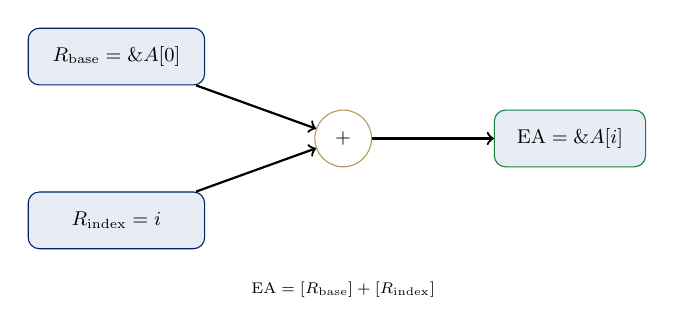
\begin{tikzpicture}[scale=0.8, transform shape,
        every node/.style={font=\small}]
      \node[draw=primary-blue, fill=light-bg, rounded corners,
            minimum width=2.8cm, minimum height=0.9cm, align=center] (Rbase) at (0,1.3) {$R_{\text{base}} = \&A[0]$};
      \node[draw=primary-blue, fill=light-bg, rounded corners,
            minimum width=2.8cm, minimum height=0.9cm, align=center] (Rindex) at (0,-1.3) {$R_{\text{index}} = i$};
      \node[draw=primary-gold, fill=white, circle, minimum size=0.9cm] (adder) at (3.6,0) {$+$};
      \node[draw=positive, fill=light-bg, rounded corners,
            minimum width=2.4cm, minimum height=0.9cm, align=center] (EAnode) at (7.2,0) {$\text{EA} = \&A[i]$};
      \draw[->, thick] (Rbase) -- (adder);
      \draw[->, thick] (Rindex) -- (adder);
      \draw[->, thick] (adder) -- (EAnode);
      \node[font=\scriptsize] at (3.6,-2.4) {$\text{EA} = [R_{\text{base}}] + [R_{\text{index}}]$};
    \end{tikzpicture}
  \end{center}
  \key{This is exactly how \texttt{A[i]} is compiled}: base register holds
  \texttt{\&A[0]}, index register holds \texttt{i}, hardware adds them.
\end{frame}

\begin{frame}{Socratic Check: Which Mode for \texttt{A[i]}?}
  \begin{alertblock}{Question}
    Inside a loop, the compiler must generate code for \texttt{A[i] = A[i] + 1}
    where \texttt{i} changes every iteration. Which addressing mode should it use
    for accessing \texttt{A[i]} --- and why not direct addressing?
  \end{alertblock}
  \begin{itemize}
    \item \bad{Direct addressing fails}: the address field is fixed at compile
      time, but \texttt{A[i]}'s address changes every iteration.
    \item \good{Indexed/based addressing wins}: \texttt{EA} is recomputed from a
      \emph{register} (\texttt{i}) every time, so the same instruction works for
      every loop iteration.
    \item This is why indexed addressing exists: it is the hardware primitive
      underneath every array access in every high-level language.
  \end{itemize}
\end{frame}

\begin{frame}{Autoincrement / Autodecrement Addressing}
  \begin{exampleblock}{Idiom: streaming through an array, or push/pop}
    \texttt{ADD R1, (R2)+} \quad $\Rightarrow$ \quad use \texttt{[R2]} as \texttt{EA},
    \emph{then} increment \texttt{R2} by the operand size.
  \end{exampleblock}
  \begin{itemize}
    \item Register-indirect \emph{plus} an automatic $\pm 1$ (or $\pm$ operand size)
      on the register, as a side effect of the instruction.
    \item Autoincrement steps forward (array traversal, stack pop); autodecrement
      steps backward (stack push).
    \item No separate ``increment'' instruction needed --- one fewer instruction per
      loop iteration.
  \end{itemize}
\end{frame}

\begin{frame}{Addressing Modes: Side by Side}
  \footnotesize
  \begin{tabular}{@{}p{2.6cm}p{2.9cm}p{2.6cm}p{3.6cm}@{}}
    \toprule
    \textbf{Mode} & \textbf{Syntax} & \textbf{EA} & \textbf{Typical use} \\
    \midrule
    Immediate        & \texttt{\#5}     & --- (value in instr.) & Constants \\
    Direct            & \texttt{1000}    & $A$                    & Global variables \\
    Indirect          & \texttt{(1000)}  & $M[A]$                 & Pointers via memory \\
    Register          & \texttt{R2}      & --- (value in reg.)   & Local variables \\
    Register-indirect  & \texttt{(R2)}    & $[R2]$                 & Pointer variables \\
    Displacement       & \texttt{d(R2)}   & $[R2] + d$             & Array elements, structs \\
    Autoincrement      & \texttt{(R2)+}   & $[R2]$, then $R2 {+}{=} n$ & Array streaming, stack pop \\
    \bottomrule
  \end{tabular}
  \vspace{0.2cm}
  \begin{center}
    \muted{Every row exists because some code idiom needs it --- not to be memorized in isolation.}
  \end{center}
\end{frame}

\begin{frame}{Worked Example: Computing \texttt{EA} by Hand}
  \begin{block}{Instruction}
    \texttt{LOAD R1, 20(R2)} \quad (displacement addressing), given $[\text{R2}] = 1000$
  \end{block}
  \begin{enumerate}
    \item Addressing mode: displacement $\Rightarrow$ $\text{EA} = [\text{R2}] + d$.
    \item Displacement field: $d = 20$.
    \item $\text{EA} = 1000 + 20 = 1020$.
    \item Operand fetched from $M[1020]$; result placed in \texttt{R1}.
  \end{enumerate}
  \begin{exampleblock}{Cost accounting}
    One register read (to get \texttt{[R2]}) $+$ one memory read (to get
    $M[\text{EA}]$) $=$ cheaper than indirect addressing's two \emph{memory} reads.
  \end{exampleblock}
\end{frame}

\transitionslide{Addressing modes tell the CPU WHERE. Now: what hardware moves the data?}

% =============================================================================
% ACT 2 --- CPU ORGANIZATION
% =============================================================================
\section{CPU Organization}

\begin{frame}{From ``Where'' to ``How''}
  \begin{block}{The next question}
    An instruction like \texttt{ADD R1, R2, R3} needs a register file, an ALU, and
    a \emph{path} connecting them so operands can travel from registers to the ALU
    and results can travel back. How much wiring do we build --- and what does
    that choice cost us?
  \end{block}
  Two architectural choices dominate this design space:
  \begin{itemize}
    \item \key{Single-bus organization} --- one shared path, everything takes turns.
    \item \key{Multiple-bus organization} --- several parallel paths, more can
      happen per clock cycle.
  \end{itemize}
  We will build both, trace the same instruction through each, and count cycles.
\end{frame}

\begin{frame}{The CPU's Internal Building Blocks}
  \begin{center}
    % Diagram: generic CPU internal organization, establishing shot before the
    % single-bus / multi-bus detail. Not to be confused with the datapath
    % diagrams that follow -- this is deliberately low-detail.
    % Coordinates: (x, y)
    %   CU  at (0, 0)    -- Control Unit
    %   ALU at (2.6, 0)  -- ALU
    %   REG at (5.2, 0)  -- Register file
    %   bus at y = -1.1  -- short internal bus segment, x in [-1.0, 6.1]
    %   MEM at (8.6, 0)  -- MAR/MDR + Main Memory, right of REG
    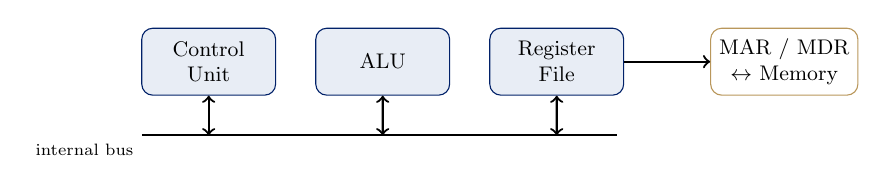
\begin{tikzpicture}[scale=0.85, transform shape,
        every node/.style={font=\small}]
      \node[draw=primary-blue, fill=light-bg, rounded corners,
            minimum width=2.0cm, minimum height=1.0cm, align=center] (CU) at (0,0) {Control\\Unit};
      \node[draw=primary-blue, fill=light-bg, rounded corners,
            minimum width=2.0cm, minimum height=1.0cm, align=center] (ALU) at (2.6,0) {ALU};
      \node[draw=primary-blue, fill=light-bg, rounded corners,
            minimum width=2.0cm, minimum height=1.0cm, align=center] (REG) at (5.2,0) {Register\\File};
      \draw[thick] (-1.0,-1.1) -- (6.1,-1.1);
      \node[font=\scriptsize, below left] at (-1.0,-1.1) {internal bus};
      \draw[<->, thick] (CU.south) -- (0,-1.1);
      \draw[<->, thick] (ALU.south) -- (2.6,-1.1);
      \draw[<->, thick] (REG.south) -- (5.2,-1.1);
      \node[draw=primary-gold, fill=white, rounded corners,
            minimum width=2.2cm, minimum height=1.0cm, align=center] (MEM) at (8.6,0) {MAR / MDR\\$\leftrightarrow$ Memory};
      \draw[->, thick] (REG.east) -- (MEM.west);
    \end{tikzpicture}
  \end{center}
  Everything on the next several slides zooms into the box you have not seen yet:
  \emph{how the register file, ALU, and buses actually wire together}.
\end{frame}

\begin{frame}{Notation: Register Transfer Language (RTL)}
  \begin{block}{RTL notation (added to the course registry)}
    \begin{itemize}
      \item $\text{R1} \gets [\text{R2}]$ \quad reads as: ``the contents of R2 are
        transferred into R1.''
      \item $[\text{X}]$ always means \emph{contents of} X (a register or memory cell).
      \item $M[\text{EA}]$ means the memory cell at address \texttt{EA}.
      \item A \key{control step} (written $T_1, T_2, \dots$) is one clock cycle's
        worth of RTL transfers.
    \end{itemize}
  \end{block}
  We will use RTL to trace instructions through hardware for the rest of this
  lecture, and again in Week 6 when we build the control unit that
  \emph{generates} these $T_1, T_2, \dots$ sequences automatically.
\end{frame}

\begin{frame}{Socratic Check: One Bus, or Many?}
  \begin{alertblock}{Design question}
    \texttt{ADD R1, R2, R3} needs two register values to reach the ALU and one
    result to come back. If every register and the ALU share a \emph{single} path,
    can two register values reach the ALU in the same clock cycle?
  \end{alertblock}
  \begin{itemize}
    \item If the answer is no, the instruction needs \emph{multiple} clock cycles
      just to move data around --- before the ALU even computes anything extra.
    \item If we instead give the ALU two dedicated input paths, one instruction
      could complete data movement in a single cycle --- at the cost of more wires.
  \end{itemize}
  Let's build both and count.
\end{frame}

\transitionslide{Design 1: everything shares ONE bus.}

% =============================================================================
% ACT 3 --- SINGLE-BUS ORGANIZATION
% =============================================================================
\section{Single-Bus Organization}

\begin{frame}{The Single-Bus Datapath}
  \begin{center}
    % Diagram: single common-bus CPU datapath (Mano-style).
    % Coordinates: (x, y)
    %   Top registers (y=2, box 1.8w x 0.9h except Rfile 2.2w):
    %     PC at (0,2)  MAR at (2.6,2)  IR at (5.2,2)  Rfile "R0..R3" at (7.8,2)
    %   Common bus: horizontal line y=0, x in [-1.0, 10.8]
    %   Bus taps (vertical arrows, above bus): x = 0, 2.6, 5.2, 7.8 (one per top reg)
    %   Y register at (3.8,-1.6) -- dedicated bus tap, buffers ALU operand 1
    %   ALU box at (5.2,-3.2) -- inputs from Y (left) and a direct bus tap at x=6.5
    %   Z register at (5.2,-4.8) -- buffers ALU result before write-back
    %   Feedback path: Z -> down to y=-5.7 -> right to x=10.5 -> up into bus
    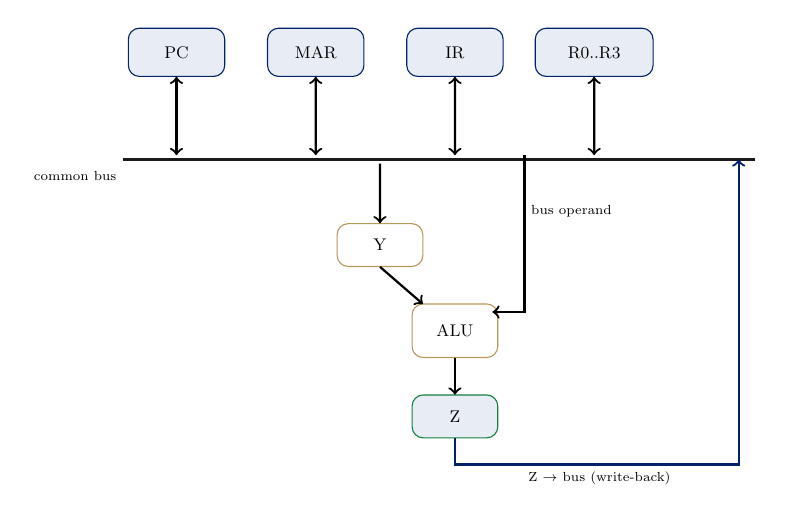
\begin{tikzpicture}[scale=0.68, transform shape,
        every node/.style={font=\small}]
      % top registers
      \node[draw=primary-blue, fill=light-bg, rounded corners,
            minimum width=1.8cm, minimum height=0.9cm, align=center] (PC) at (0,2) {PC};
      \node[draw=primary-blue, fill=light-bg, rounded corners,
            minimum width=1.8cm, minimum height=0.9cm, align=center] (MAR) at (2.6,2) {MAR};
      \node[draw=primary-blue, fill=light-bg, rounded corners,
            minimum width=1.8cm, minimum height=0.9cm, align=center] (IR) at (5.2,2) {IR};
      \node[draw=primary-blue, fill=light-bg, rounded corners,
            minimum width=2.2cm, minimum height=0.9cm, align=center] (RF) at (7.8,2) {R0..R3};
      % common bus
      \draw[very thick, jet] (-1.0,0) -- (10.8,0);
      \node[font=\scriptsize, below left] at (-1.0,-0.1) {common bus};
      % taps: top registers to bus
      \draw[<->, thick] (PC.south) -- (0,0.08);
      \draw[<->, thick] (MAR.south) -- (2.6,0.08);
      \draw[<->, thick] (IR.south) -- (5.2,0.08);
      \draw[<->, thick] (RF.south) -- (7.8,0.08);
      % Y register
      \node[draw=primary-gold, fill=white, rounded corners,
            minimum width=1.6cm, minimum height=0.8cm, align=center] (Y) at (3.8,-1.6) {Y};
      \draw[->, thick] (3.8,-0.08) -- (Y.north);
      % ALU (plain rectangle, low-risk shape)
      \node[draw=primary-gold, fill=white, rounded corners,
            minimum width=1.6cm, minimum height=1.0cm, align=center] (ALU) at (5.2,-3.2) {ALU};
      \draw[->, thick] (Y.south) -- (4.6,-2.7);
      \draw[->, thick] (6.5,0.08) |- (5.9,-2.85);
      \node[font=\scriptsize, above right] at (6.5,-1.2) {bus operand};
      % Z register
      \node[draw=positive, fill=light-bg, rounded corners,
            minimum width=1.6cm, minimum height=0.8cm, align=center] (Z) at (5.2,-4.8) {Z};
      \draw[->, thick] (ALU.south) -- (Z.north);
      % feedback Z -> bus
      \draw[->, thick, primary-blue] (5.2,-5.2) -- (5.2,-5.7) -- (10.5,-5.7) -- (10.5,0);
      \node[font=\scriptsize, below] at (7.9,-5.7) {Z $\to$ bus (write-back)};
    \end{tikzpicture}
  \end{center}
  \cite{Mano1993_computer_system_architecture}
\end{frame}

\begin{frame}{How the Single Bus Works}
  \begin{block}{The core constraint}
    Only \emph{one} value can be on the bus at any instant. Every transfer between
    registers happens \emph{through} the bus, one at a time.
  \end{block}
  \begin{itemize}
    \item The ALU needs \emph{two} inputs, but the bus can only deliver one value
      per cycle --- so one operand must be parked somewhere while the second
      arrives. That is what the hidden register \texttt{Y} is for.
    \item \texttt{Z} holds the ALU's result until it can be written back onto the
      bus (the bus is busy carrying the second operand at the moment the ALU computes).
    \item Consequence: a two-operand operation takes \emph{multiple} control steps,
      not one.
  \end{itemize}
\end{frame}

\begin{frame}{Worked Trace: \texttt{R1} $\gets$ \texttt{R2 + R3} on a Single Bus}
  \footnotesize
  \begin{tabular}{@{}clll@{}}
    \toprule
    \textbf{Step} & \textbf{RTL} & \textbf{On the bus} & \textbf{What happens} \\
    \midrule
    $T_1$ & $Y \gets [R2]$            & $[R2]$      & R2 onto bus, latched into Y \\
    $T_2$ & $Z \gets [Y] + [R3]$      & $[R3]$      & R3 onto bus $\to$ ALU; ALU adds $Y$; result $\to Z$ \\
    $T_3$ & $R1 \gets [Z]$            & $[Z]$       & Z onto bus, latched into R1 \\
    \bottomrule
  \end{tabular}
  \vspace{0.3cm}
  \begin{alertblock}{Running total}
    \textbf{3 control steps} for one \texttt{ADD} on the single-bus organization.
    Keep this number --- we compare it to the multi-bus trace shortly.
  \end{alertblock}
\end{frame}

\begin{frame}{Why \texttt{Y} and \texttt{Z} Exist}
  \begin{itemize}
    \item \texttt{Y} exists because the bus can carry only one operand per cycle,
      but the ALU needs two simultaneously --- \texttt{Y} \emph{remembers} the
      first one while the second is still in transit.
    \item \texttt{Z} exists because the ALU's result cannot be written back to the
      bus in the \emph{same} cycle the bus is occupied by the second operand ---
      \texttt{Z} \emph{holds} the result for one extra step.
    \item Both are the direct hardware cost of sharing one bus: every two-operand
      instruction pays for buffering.
  \end{itemize}
\end{frame}

\begin{frame}{Single-Bus Organization: Trade-offs}
  \begin{block}{Cost vs.\ speed}
    \begin{itemize}
      \item \good{Pro}: one bus $=$ one set of wires and multiplexers --- cheapest
        to build, easiest to extend with new registers.
      \item \good{Pro}: simple, uniform control logic (every transfer looks the same).
      \item \bad{Con}: every multi-operand instruction takes several control steps
        --- more clock cycles per instruction, so lower throughput.
      \item \bad{Con}: needs the extra \texttt{Y}/\texttt{Z} buffering hardware
        around the ALU.
    \end{itemize}
  \end{block}
\end{frame}

\begin{frame}{Socratic Check: Counting Cycles}
  \begin{alertblock}{Question}
    If every bus transfer takes exactly one clock cycle, how many cycles does
    \texttt{R1} $\gets$ \texttt{R2 + R3} take on the single-bus organization we just
    traced?
  \end{alertblock}
  \begin{itemize}
    \item Count the control steps in the trace: $T_1, T_2, T_3$.
    \item \key{Answer: 3 cycles} --- one to stage the first operand, one to stage
      the second \emph{and} compute, one to write back the result.
    \item Hold onto this number. We are about to see a design that does the same
      job in one cycle.
  \end{itemize}
\end{frame}

\transitionslide{Design 2: give the ALU dedicated inputs.}

% =============================================================================
% ACT 4 --- MULTIPLE (THREE-)BUS ORGANIZATION
% =============================================================================
\section{Multiple-Bus Organization}

\begin{frame}{The Three-Bus Datapath}
  \begin{center}
    % Diagram: three-bus CPU datapath (Hamacher-style).
    % Coordinates: (x, y)
    %   Rfile box at (0,0), width 2.0, height 2.6 -- register file, 2 read ports + 1 write port
    %   ALU box at (4.2,0), width 1.4, height 1.4
    %   Bus A: Rfile upper-east tap (1.0,0.6) -> ALU upper-west input (3.5,0.45)
    %   Bus B: Rfile lower-east tap (1.0,-0.6) -> ALU lower-west input (3.5,-0.45)
    %   Bus C: ALU east (4.9,0) -> down to y=-2.2 -> left to x=0 -> up into Rfile.south
    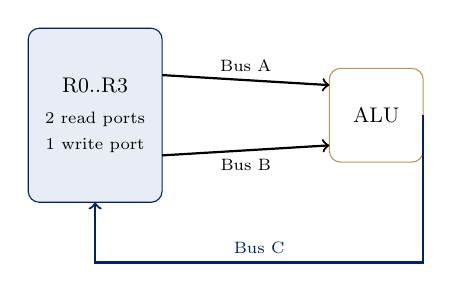
\begin{tikzpicture}[scale=0.85, transform shape,
        every node/.style={font=\small}]
      \node[draw=primary-blue, fill=light-bg, rounded corners,
            minimum width=2.0cm, minimum height=2.6cm, align=center] (RF) at (0,0) {R0..R3\\[2pt]\scriptsize 2 read ports\\\scriptsize 1 write port};
      \node[draw=primary-gold, fill=white, rounded corners,
            minimum width=1.4cm, minimum height=1.4cm, align=center] (ALU) at (4.2,0) {ALU};
      \draw[->, thick] (1.0,0.6) -- node[midway, above, font=\scriptsize] {Bus A} (3.5,0.45);
      \draw[->, thick] (1.0,-0.6) -- node[midway, below, font=\scriptsize] {Bus B} (3.5,-0.45);
      \draw[->, thick, primary-blue] (4.9,0) -- (4.9,-2.2) -- (0,-2.2) node[midway, above, font=\scriptsize]{Bus C} -- (0,-1.3);
    \end{tikzpicture}
  \end{center}
  \key{Bus A and Bus B} read two \emph{different} registers in the \emph{same}
  cycle; \key{Bus C} writes the ALU's result back \cite{Hamacher2002_computer_organization}.
\end{frame}

\begin{frame}{Worked Trace: \texttt{R1} $\gets$ \texttt{R2 + R3} on Three Buses}
  \footnotesize
  \begin{tabular}{@{}clll@{}}
    \toprule
    \textbf{Step} & \textbf{RTL} & \textbf{On the buses} & \textbf{What happens} \\
    \midrule
    $T_1$ & $R1 \gets [R2] + [R3]$ & $A{=}[R2]$, $B{=}[R3]$, $C{=}\text{result}$ &
      Both operands read \emph{and} the ALU output written back, all in one cycle \\
    \bottomrule
  \end{tabular}
  \vspace{0.3cm}
  \begin{alertblock}{Running total}
    \textbf{1 control step} for the same \texttt{ADD} --- versus \textbf{3} on the
    single-bus organization. Same instruction, same ALU, different wiring.
  \end{alertblock}
\end{frame}

\begin{frame}{Why Three Buses Are Faster}
  \begin{itemize}
    \item Bus A and Bus B are \emph{separate physical paths} --- the register file
      can put two different registers' contents on them \emph{simultaneously}.
    \item The ALU no longer needs a \texttt{Y} buffer: both inputs arrive in the
      same cycle, directly from the register file.
    \item Bus C lets the result be written back \emph{in the same cycle} it is
      computed, since it is not competing with Bus A/B for the same wire.
    \item Net effect: the sequential bottleneck from the single-bus design simply
      does not exist here.
  \end{itemize}
\end{frame}

\begin{frame}{Three-Bus Organization: Trade-offs}
  \begin{block}{Cost vs.\ speed}
    \begin{itemize}
      \item \good{Pro}: most two-operand register instructions complete data
        movement in a single control step.
      \item \good{Pro}: no \texttt{Y}/\texttt{Z} buffering needed for the common case.
      \item \bad{Con}: three times the bus wiring, plus the multiplexers needed to
        route any register onto any of the three buses.
      \item \bad{Con}: more complex control logic --- three buses must be driven
        correctly every cycle, not just one.
    \end{itemize}
  \end{block}
\end{frame}

\begin{frame}{Single-Bus vs.\ Three-Bus: The Full Comparison}
  \footnotesize
  \begin{tabular}{@{}p{3.2cm}p{4.4cm}p{4.4cm}@{}}
    \toprule
     & \textbf{Single bus} & \textbf{Three bus} \\
    \midrule
    Wiring cost        & Low (one bus)                & High (three buses $+$ muxes) \\
    Cycles for $R1 \gets R2{+}R3$ & 3 ($T_1, T_2, T_3$)   & 1 ($T_1$) \\
    Extra registers needed & Y, Z (buffering)         & None (common case) \\
    Control logic       & Simple, uniform              & More complex, more signals \\
    Best fit             & Cost-sensitive designs        & Performance-sensitive designs \\
    \bottomrule
  \end{tabular}
  \vspace{0.3cm}
  \begin{center}
    \muted{Neither design is ``correct'' --- they sit at different points on the
    same cost/speed trade-off curve.}
  \end{center}
\end{frame}

\begin{frame}{Socratic Check: Why Not \emph{N} Buses?}
  \begin{alertblock}{Question}
    If three buses beat one, why not build a CPU with ten buses, or a hundred?
  \end{alertblock}
  \begin{itemize}
    \item Every additional bus needs its own wiring \emph{and} its own multiplexer
      logic at every register --- cost grows roughly with the number of buses,
      not for free.
    \item Most instructions only need two operand reads and one result write ---
      beyond three buses, there is little left to parallelize \emph{within a single
      instruction}.
    \item Real speedups beyond this point come from a different idea entirely:
      \emph{overlapping different instructions} in time --- which is exactly what
      pipelining (Week 11) does.
  \end{itemize}
\end{frame}

% =============================================================================
% ACT 5 --- SYNTHESIS
% =============================================================================
\section{Synthesis}

\begin{frame}{The Two Threads Meet}
  \begin{block}{Addressing modes have a bus-organization cost too}
    Recall indirect addressing: \emph{two} memory reads to resolve \texttt{EA}.
    On a single-bus CPU, each of those reads is itself another multi-step bus
    transaction --- the ``expensive'' addressing modes and the ``expensive''
    bus organization compound.
  \end{block}
  \begin{itemize}
    \item Cheap addressing (immediate, register) $+$ cheap bus (single) $=$ minimal
      hardware, more cycles per instruction.
    \item Expensive addressing (indirect) $+$ expensive bus (three-bus) can still
      be fast, but every design choice is paid for in wires or in cycles ---
      never free.
  \end{itemize}
\end{frame}

\begin{frame}{Bridge to Week 6}
  \begin{block}{What we built today}
    \begin{itemize}
      \item Seven addressing modes, each motivated by a real code idiom.
      \item A single-bus datapath, traced step by step: 3 control steps for
        \texttt{R1} $\gets$ \texttt{R2+R3}.
      \item A three-bus datapath, same instruction: 1 control step.
    \end{itemize}
  \end{block}
  \begin{exampleblock}{What's still missing}
    We wrote $T_1, T_2, T_3$ by hand. \key{Something has to generate that sequence
    automatically}, for \emph{every} instruction in the ISA, every time it runs.
    That ``something'' is the \textbf{control unit} --- hardwired control, next week.
  \end{exampleblock}
\end{frame}

\begin{frame}{Summary}
  \begin{itemize}
    \item \key{Addressing mode} $=$ the rule for computing \texttt{EA} from an
      instruction's address field; each mode trades flexibility against extra
      memory/bus reads.
    \item \key{RTL notation} ($R \gets [\cdot]$, $M[\text{EA}]$, control steps
      $T_1, T_2, \dots$) is how we describe hardware-level data movement precisely.
    \item \key{Single-bus organization}: cheap wiring, sequential transfers, needs
      \texttt{Y}/\texttt{Z} buffering, more cycles per instruction.
    \item \key{Multiple-bus organization}: parallel register reads and writes,
      fewer cycles per instruction, more wiring and control complexity.
    \item Same instruction, same ALU, different wiring $\Rightarrow$ 3 cycles vs.\ 1
      --- the cost/speed trade-off, made concrete.
  \end{itemize}
\end{frame}

\begin{frame}{References}
  \footnotesize
  \bibliographystyle{plain}
  \bibliography{../Bibliography_base}
\end{frame}

\end{document}
